%! Author = gra
%! Date = 24.03.24

% Preamble
\begin{flushleft}
    \subsection{Analyse gängiger PostgreSQL HA Cluster Lösungen}
    Auf dem Markt existieren eine Reihe von Clusterlösungen für PostgreSQL.\\
    Folgende werden analysiert und anschliessend einer Vorauswahl unterzogen:
    \begin{table}[H]


\begin{tabular}{lll}
\toprule
Anbieter & Lösung & Systemart \\
\midrule
Percona & Patroni & Monolitisch \\
EnterpriseDB & Patroni & Monolitisch \\
KSGR Lösung & Eigenes System & Monolitisch \\
The Pgpool Global Development Group & pgpool-II & Monolitisch \\
hapostgres & pg\_auto\_failover & Monolitisch \\
EnterpriseDB & CloudNativePG & Monolitisch \\
Zalando SE. & Patroni & Monolitisch \\
OnGres, Inc. & StackGres & Monolitisch / Distributed SQL \\
Citus Data, a Microsoft Company & Citus & Distributed SQL \\
Yugabyte, Inc. & YugabyteDB & Distributed SQL \\
\bottomrule
\end{tabular}
\caption{Anbieter und Systeme} \label{solution_list}
\end{table}

    %! Author = gra
%! Date = 24.03.24

% Preamble
\begin{flushleft}
    \subsubsection{Percona}
    Percona bietet nebst dem bekannteren Galera-Cluster und \Gls{MySQL}- und \Gls{MariaDB}\\
    auch Dienstleistungen \cite{WEM9KYAX} aller Art für PostgreSQL an.
\end{flushleft}
\begin{flushleft}
    Percona arbeitet oft auf Basis von Patroni,\\
    bietet aber auch eigene Erweiterungen und eigene Software an\cite{66AS3BU9}.
\end{flushleft}
\begin{flushleft}
    Da Percona keine Open-Source-Lösungen bietet, sondern Service-orientiert ist,\\
    wird Percona nicht betrachtet.\\
    Allerdings wird immer mal wieder auf frei zugängliche Dokumentationen von Percona verwiesen werden.
\end{flushleft}
    %! Author = gra
%! Date = 24.03.24

% Preamble
\begin{flushleft}
    \subsubsection{EnterpriseDB}
    EnterpriseDB, oder EDB, ist ein führendes Software- und Servicehaus für PostgreSQL\cite{UIY9LXTF}.\\
    Nebst Dienstleistungen für das Management von PostgreSQL-Umgebungen, Migrationen aus Oracle-Umgebungen und anderem,\\
    bietet EDB auch eine vielwahl an zusätzlicher Software und eigene Replikationslösungen.\\
\end{flushleft}
\begin{flushleft}
    EDB bietet PostgreSQL auf Kubernetes mittels CloudNativePG an,\\
    hat aber auch eine eigens Entwickelte Distributed SQL / Active-Active Lösung an.
\end{flushleft}
\begin{flushleft}
    Da die EDB-Lösungen nicht Open-Source sind resp. von EDB aufgekaufte Lösungen nicht mehr ohne Subscription betreibbar sind,\\
    werden sie nicht berücksichtigt.
    Allerdings wird immer mal wieder auf frei zugängliche Dokumentationen von EDB verwiesen werden.
\end{flushleft}
%    %! Author = itgramic
%! Date = 05.12.23

% Preamble
\subsubsection{\Gls{PostgreSQL} Replikation}
PostgreSQL bietet von Haus aus Möglichkeiten, um Replikationen durchzuführen.
Dabei ist nicht jede gleich gut für jedes Szenario geeignet\cite{FZAHA89U}.
    %! Author = itgramic
%! Date = 05.12.23

% Preamble
\subsubsection{KSGR Lösung}
Das Kantonsspital Graubünden hat basierend auf \gls{keepalived} wird geprüft ob die primäre Seite erreichbar und betriebsbereit ist.
Trifft dies nicht mehr zu, wird ein \Gls{Failover} durchgeführt\cite{NLF2IDBZ}.
Ist die primäre Seite wieder verfügbar, wird ein Restore auf die primäre Seite gefahren.

Es wird beim Restore immer ein komplettes Backup der sekundären Seite auf die primäre Seite übertragen.
Ursache ist, dass die normalerweise für den Datenrestore benötigten \Gls{PostgreSQL} Board mittel nur für eine relativ kurze Zeit eingesetzt werden können ehe die differenzen zwischen den beiden Seiten zu gross werden.

Bei kleinen Datenbanken wie jene für \Gls{Harbor} und \Gls{GitLab} ist die Zeit die hierfür benötigt wird, nicht relevant.
Sind die Datenbanken auf dem \Gls{PostgreSQL Cluster} jedoch grösser, kann der Restore mehrere Minuten dauern.
    %! Author = itgramic
%! Date = 05.12.23

% Preamble
\subsubsection{pgpool-II}
\begin{flushleft}
    pgpool-II ist eine Middleware die zwischen einem \Gls{PostgreSQL Cluster} und einem PostgreSQL-Client gesetzt wird.
\end{flushleft}
\begin{flushleft}
    \paragraph{Core-Features}
    pgpool-II bietet folgende Core-Feature\cite{3XWCD3KX}:
    \begin{itemize}
        \item Watchdog für Automatischer Failover
        \item Eigener \Gls{Quorum}-Algorithmus
        \item Integrierter \Gls{Connection Pooler}
        \item Eigenes Replikationssystem
        \item Integriertes Load Balancing
        \item Limiting Exceeding Connections, also queuen von Connections
        \item In Memory Query Caching
        \item Online Node Recovery / Resynchronisation
    \end{itemize}
\end{flushleft}
\begin{flushleft}
    \paragraph{Replikation}
    pgpool-II bietet ein eigenes Replikationssystem an.
\end{flushleft}
\begin{flushleft}
    Es besteht allerdings die Möglichkeit, die PostgreSQL-Standardreplikationen zu verwenden.
\end{flushleft}
\begin{flushleft}
    \paragraph{Proxy}
    pgpool-II hat bereits einen intergrierten Load Balancer.\\
    Einen zusätzlichen Proxy wird daher nicht benötigt.
\end{flushleft}
\begin{flushleft}
    \paragraph{Pooling}
    pgpool-II bietet ebenfalls von Haus aus einen \Gls{Connection Pooler}.
\end{flushleft}
\begin{flushleft}
    \paragraph{API / Skripte}
    pgpool-II bietet mit \texttt{pgpool} ein eigenes Command- und Toolset an.\\
    Mit dem CLI-Tool \texttt{pcp\_command} bietet pgpool-II zudem über eine abgesicherte API,\\
    die auch via Netzwerk erreichbar ist.
\end{flushleft}
\begin{flushleft}
    \paragraph{Maintenance}
    pgpool-II hat kein GitLab- oder GitHub-Repository.
    Metriken wie die GitHub Insights, welche Aufschluss über den Zustand des Projekts geben, finden sich nicht.
\end{flushleft}
\begin{flushleft}
    Die Dokumentation wird zwar aktualisiert, ist aber sehr minimalistisch gehalten.\\
    Sie bietet nur wenig Informationen zum Aufbau und Architektur von pgpool-II.
\end{flushleft}


    %! Author = itgramic
%! Date = 05.12.23

% Preamble
\clearpage
\begin{flushleft}
    \subsubsection{pg\_auto\_failover}
    pg\_auto\_failover ist eine PostgreSQL-Erweiterung, die von der Microsoft Subunternehmen Citus Data entwickelt wird.
\end{flushleft}
\begin{flushleft}
    \paragraph{Core-Features}
    Die wichtigsten Features von pg\_auto\_failover sind:
    \begin{itemize}
        \item API
        \item PostgreSQL Extension, also reines PostgreSQL
        \item State Machine Driven
        \item Replikations-Quorum
        \item Citus kompatibel
        \item Azure VM Support
    \end{itemize}
\end{flushleft}
\begin{flushleft}
    \paragraph{Replikation}
    pg\_auto\_failover bietet die Standard PostgreSQL-Replikationen.
\end{flushleft}
\begin{flushleft}
    \paragraph{Proxy}
    pg\_auto\_failover benötigt einen \Gls{HAProxy}, um Load Balancing betreiben zu können  \cite{VYXTI7BS}.
\end{flushleft}
\begin{flushleft}
    \paragraph{API / Skripte}
    pg\_auto\_failover bietet ein eigenes CLI-Tool, \texttt{pg\_autoctl}.
    Dieses stellt Commands für das Einbinden neuer Nodes,
    das Managen von Nodes (Maintenance resp. Switchover),\\
    Konfigurieren oder Monitoren des Systems zur Verfügung \cite{4X2AKDB6}.
\end{flushleft}
\clearpage
\begin{flushleft}
    \paragraph{Architektur}
    Die Dokumentation resp. Grafik von pg\_auto\_failover  \cite{PZZIZ5RT} zeigt auf, wie der Failover funktioniert:
    \begin{figure}[H]
        \centering
        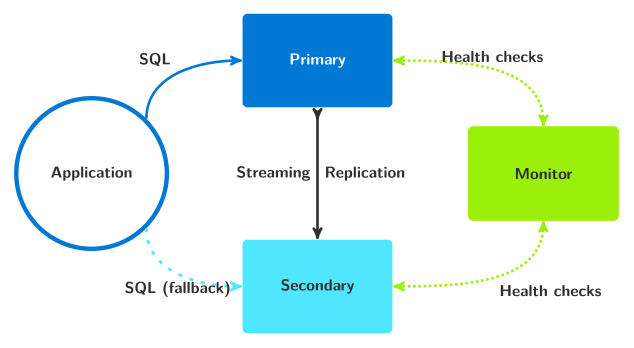
\includegraphics[width=0.75\linewidth]{source/implementation/evaluation/postgresql_ha_solutions/pg_auto_failover/pg_auto-failover_arch-single-standby}
        \caption{pg\_auto\_failover-Architektur - Single Standby}
        \label{fig:pg_auto-failover_arch-single-standby}
    \end{figure}
    Aber wie die Grafik zeigt, können auch Multi-Nodes können eingebunden werden \cite{4ZKBDG57}:
    \begin{figure}[H]
        \centering
        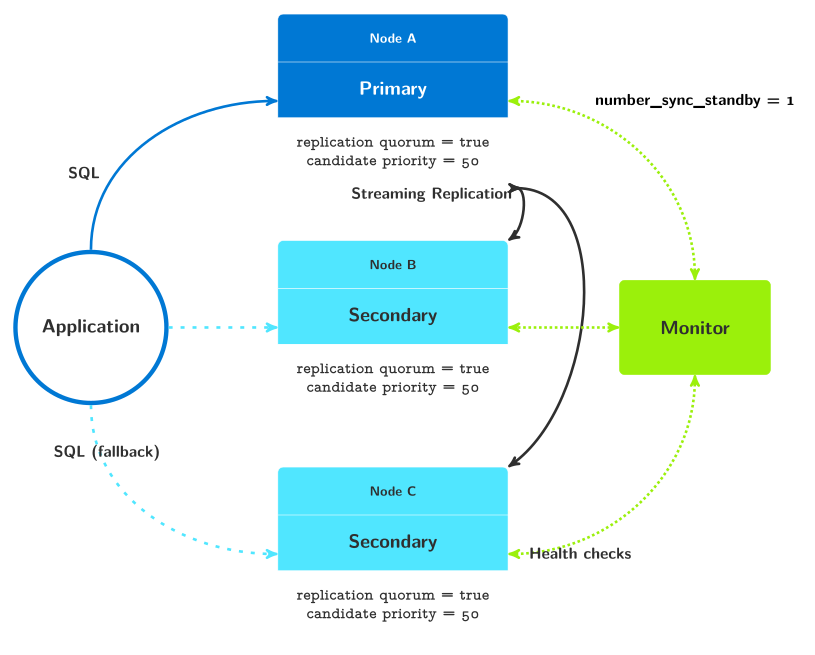
\includegraphics[width=0.75\linewidth]{source/implementation/evaluation/postgresql_ha_solutions/pg_auto_failover/pg_auto-failover_arch-multi-standby}
        \caption{pg\_auto\_failover-Architektur - Multi-Node Standby}
        \label{fig:pg_auto-failover_arch-multi-standby}
    \end{figure}
    \clearpage
    pg\_auto\_failover kann Citus einbinden.
    Allerdings bleibt die Architektur im Kern immer monolithisch.\\
    Die nachfolgende Grafik zeigt die Architektur mit Citus \cite{3FVHLIFE}:
    \begin{figure}[H]
        \centering
        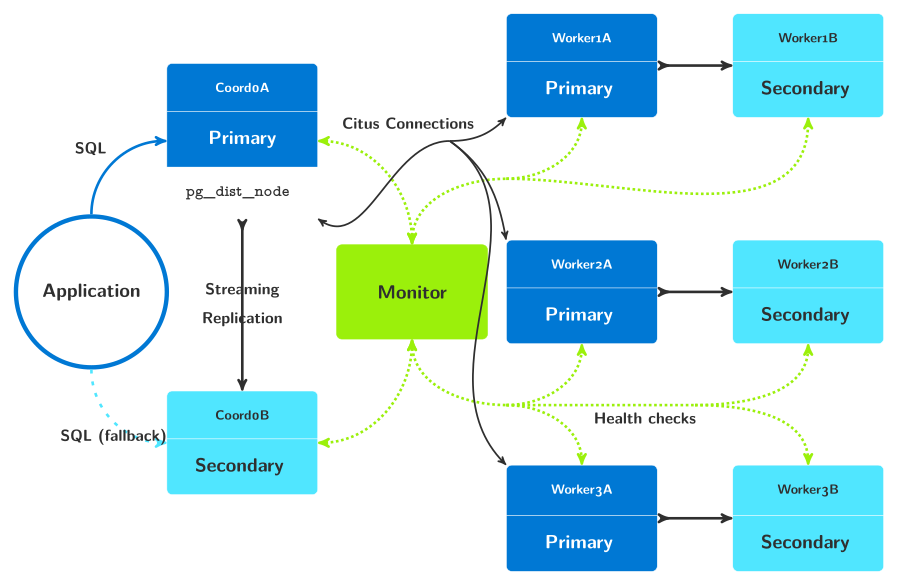
\includegraphics[width=0.75\linewidth]{source/implementation/evaluation/postgresql_ha_solutions/pg_auto_failover/pg_auto-failover_arch-citus}
        \caption{pg\_auto\_failover-Architektur - Citus}
        \label{fig:pg_auto-failover_arch-citus}
    \end{figure}
\end{flushleft}
\begin{flushleft}
    \paragraph{Synergien und Mehrwert}
    pg\_auto\_failover bietet eine Docker-Compose-Integration.\\
    Allerdings ist keine Kubernetes-Integration dokumentiert.
\end{flushleft}
\begin{flushleft}
    Damit bietet pg\_auto\_failover keine Möglichkeit\\
    Synergien zwischen monolithischer Architektur und einer Cloud-Native-Umsetzung auf Kubernetes.\\
    Entsprechend ist kein Mehrwert vorhanden.
\end{flushleft}
    %! Author = itgramic
%! Date = 05.12.23

% Preamble
\begin{flushleft}
    \subsubsection{CloudNativePG}
    CloudNativePG ist eine Containerlösung für PostgreSQL auf Kubernetes.
\end{flushleft}
\begin{flushleft}
    \paragraph{Core-Features}
    Die wichtigsten Features von CloudNativePG sind\cite{5ALQPE2U}:
    \begin{description}
        \item k8s API integration
        \item Autoamtischer Failover
        \item Self-Healing von Nodes resp. Replikas
        \item Skalierbarkeit (Vertikal, Horizontal bedingt)
        \item Volumne Backup
        \item Object Backup
        \item Rolling PostgreSQL Upgrade / Updates
        \item Pooling mit PgBouncer
        \item Offline und Online Import von bestehenden PostgreSQL DBs
    \end{description}
\end{flushleft}
\begin{flushleft}
    \paragraph{Replikation}
    CloudNativePG bietet die üblichen PostgreSQL Replikaionen an.
\end{flushleft}
\begin{flushleft}
    \paragraph{Proxy}
    CloudNativePG benötigt keinen zusätzlichen Proxy.
\end{flushleft}
\begin{flushleft}
    \paragraph{Pooling}
    CloudNativePG unterstützt pgBouncer als Pooler.
\end{flushleft}
\begin{flushleft}
    \paragraph{API / Skripte}
    CloudNativePG bietet eine API zum Monitoren und Verwalten von Backups, Clustern und dem System selbst\cite{L7PXKAUY}.
\end{flushleft}
\begin{flushleft}
    \paragraph{Architektur}
    Kubernetes regelt die Zugriffe mittels eines entsprechenden Services in die Nodes auf den Pods:
    \begin{figure}[H]
        \centering
        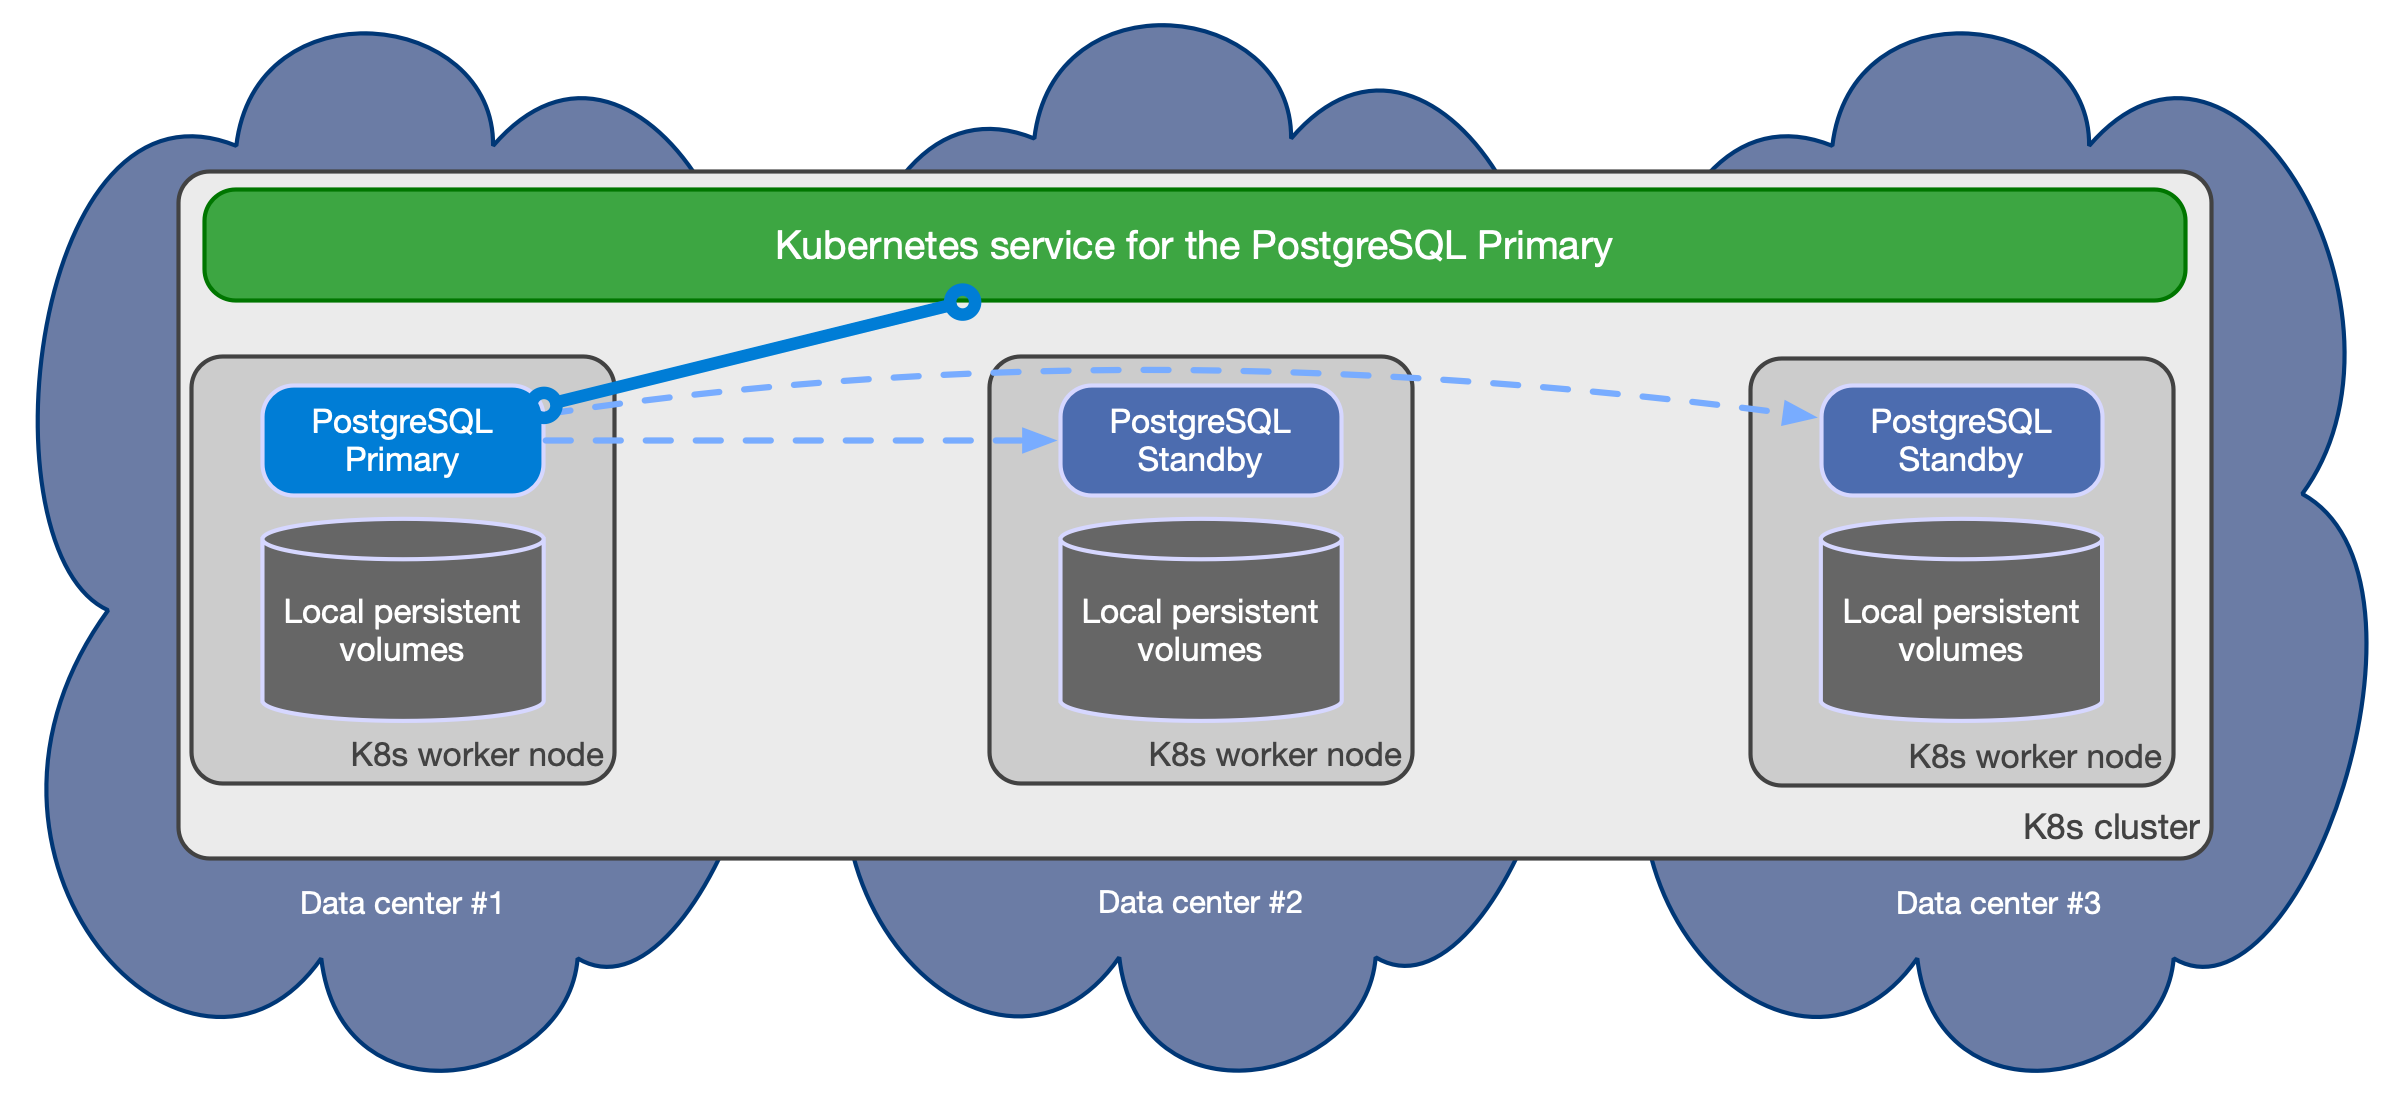
\includegraphics[width=0.75\linewidth]{source/implementation/evaluation/postgresql_ha_solutions/cloudnativepg/k8s-pg-architecture}
        \caption{CloudNativePG - Kubernetes - PostgreSQL}
        \label{fig:k8s-pg-architecture}
    \end{figure}
\end{flushleft}
\begin{flushleft}
    Dabei werden die Read-write workloads an den Primary Node gesendet:
    \begin{figure}[H]
        \centering
        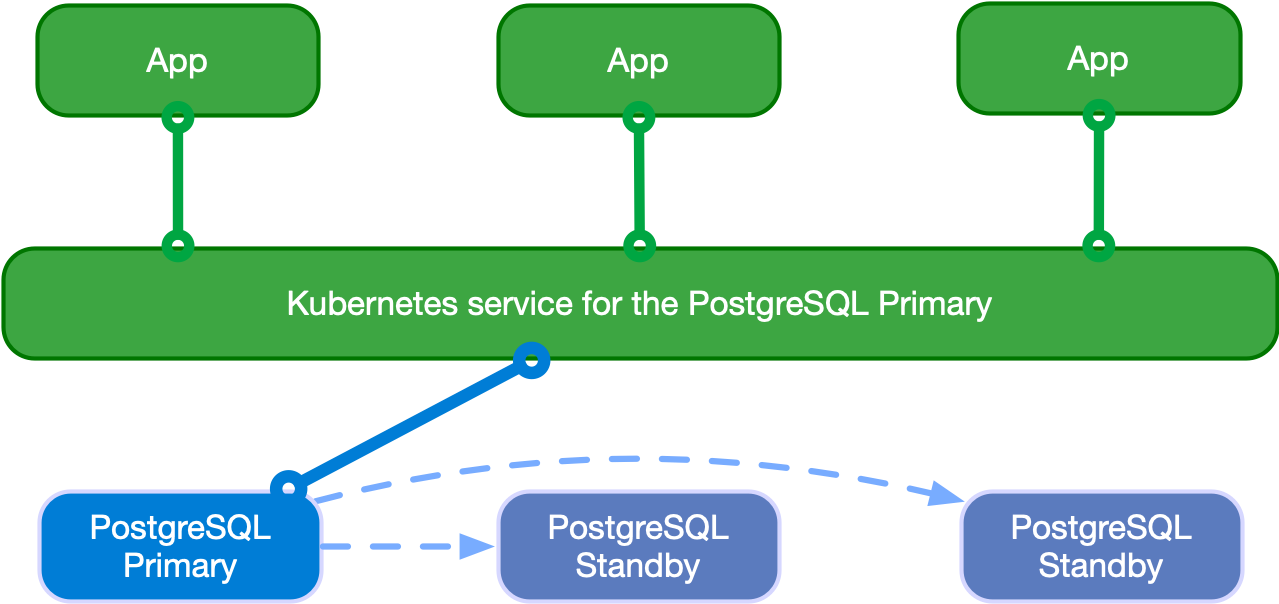
\includegraphics[width=0.75\linewidth]{source/implementation/evaluation/postgresql_ha_solutions/cloudnativepg/cloudnativepg-architecture-rw}
        \caption{CloudNativePG - Kubernetes - Read-write workloads}
        \label{fig:cloudnativepg-architecture-rw}
    \end{figure}
\end{flushleft}
\begin{flushleft}
    Read-only workloads werden mit Round robin an die Replikas zugewiesen:
    \begin{figure}[H]
        \centering
        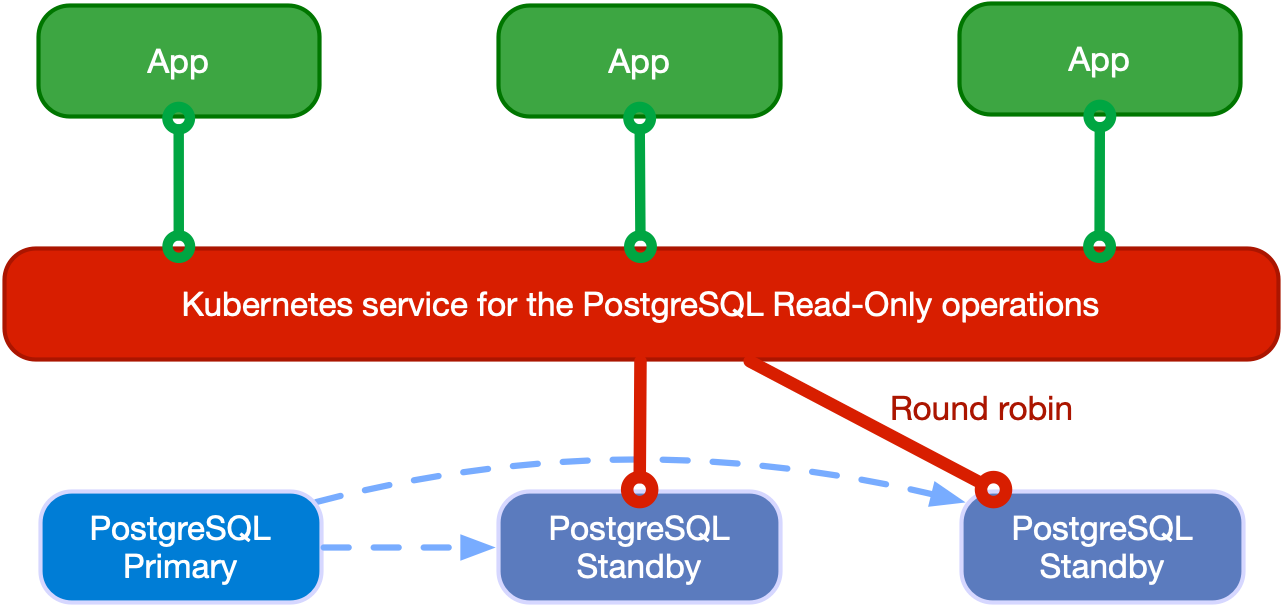
\includegraphics[width=0.75\linewidth]{source/implementation/evaluation/postgresql_ha_solutions/cloudnativepg/cloudnativepg-architecture-read-only}
        \caption{CloudNativePG - Kubernetes - Read-only workloads}
        \label{fig:cloudnativepg-architecture-read-only}
    \end{figure}
\end{flushleft}
\begin{flushleft}
    Es könnten auch Lösungen mit Designated Kubernetes-Clustern in einem anderen RZ oder einer anderen Geo-Region relaisiert werden.
\end{flushleft}
\begin{flushleft}
    \paragraph{Maintenance}
\end{flushleft}
\begin{flushleft}
    \paragraph{Synergien und Mehrwert}
    CloudNativePG bleibt ein Monolithisches System,\\welches aber keine Möglichkeit bietet,\\auch auf einem Normalen Serversetting betrieben zu werden.
\end{flushleft}
\begin{flushleft}
    Daher bietet CloudNativePG weder einen Benefit durch seine Architektur noch mit der Möglichkeit,\\Synergien nutzen zu können.
\end{flushleft}
    %! Author = itgramic
%! Date = 05.12.23

% Preamble
\clearpage
\begin{flushleft}
    \subsubsection{Patroni}
    Patroni ist eine von Zalando auf Basis von Python entwickelte HA-Lösung für \Gls{PostgreSQL}.\\
    Patroni wird aktiv von Zalando gepflegt.
\end{flushleft}
\begin{flushleft}
    \paragraph{Core-Features}
    Patroni bietet folgende Core-Features:
    \begin{itemize}
        \item Rest-API und eigenes Skript- und Toolset
        \item Aktionen und Konfigurationen im Konsensprinzip abgestimmt
        \item Manueller oder Sheduled Switchover
        \item Reines PostgreSQL als Basis, Patroni setzt Hilfe von Python darauf auf
        \item Automatische reintegration von Nodes nach einem Fehler
        \item Citus kompatibel
        \item Docker und Docker-compose Dokumentation
    \end{itemize}
\end{flushleft}
\begin{flushleft}
    \paragraph{Replikation}
    Patroni bietet per Default eine eigene Replikation an.\\
    Diese ist allerdings eine asynchrone Replikation.
\begin{flushleft}
    Patroni unterstützt aber die synchrone Replikation von \Gls{PostgreSQL}.
\end{flushleft}
\end{flushleft}
\begin{flushleft}
    \paragraph{Proxy}
    Patroni benötigt einen \Gls{HAProxy}, um Load Balancing betreiben zu können\cite{VYXTI7BS}.
\end{flushleft}
\begin{flushleft}
    \paragraph{Pooling}
    Patroni benötigt einen externen \Gls{Connection Pooler}.\\
    Hier wird oft PgBouncer \cite{ATBELZ2X} verwendet.
\end{flushleft}
\begin{flushleft}
    \paragraph{API / Skripte}
    Patroni hat ein eigenes Tool- und Commandset, \texttt{patronictl}, welches die Verwaltung vereinfacht.\\
    Es umfasst das Ändern und Erfassen von Konfigurationen, das Forcieren eines Failovers als Switchover, Maintenance Handling und Informationsbeschaffung.\\
    Zusätzlich bietet Patroni eine API, welche Daten für das Monitoring bereitstellt,\\
    aber auch Betriebsfunktionen zur Verfügung stellt.\\
\end{flushleft}
\begin{flushleft}
    \paragraph{\gls{etcd}}
    Patroni benötigt etcd oder \Gls{Consul} als \Gls{Key-Value-Store}.
\end{flushleft}
\begin{flushleft}
    \paragraph{Architektur}
    Das Architektur-Schaubild sieht folgendermassen aus:
    \begin{figure}[H]
        \centering
        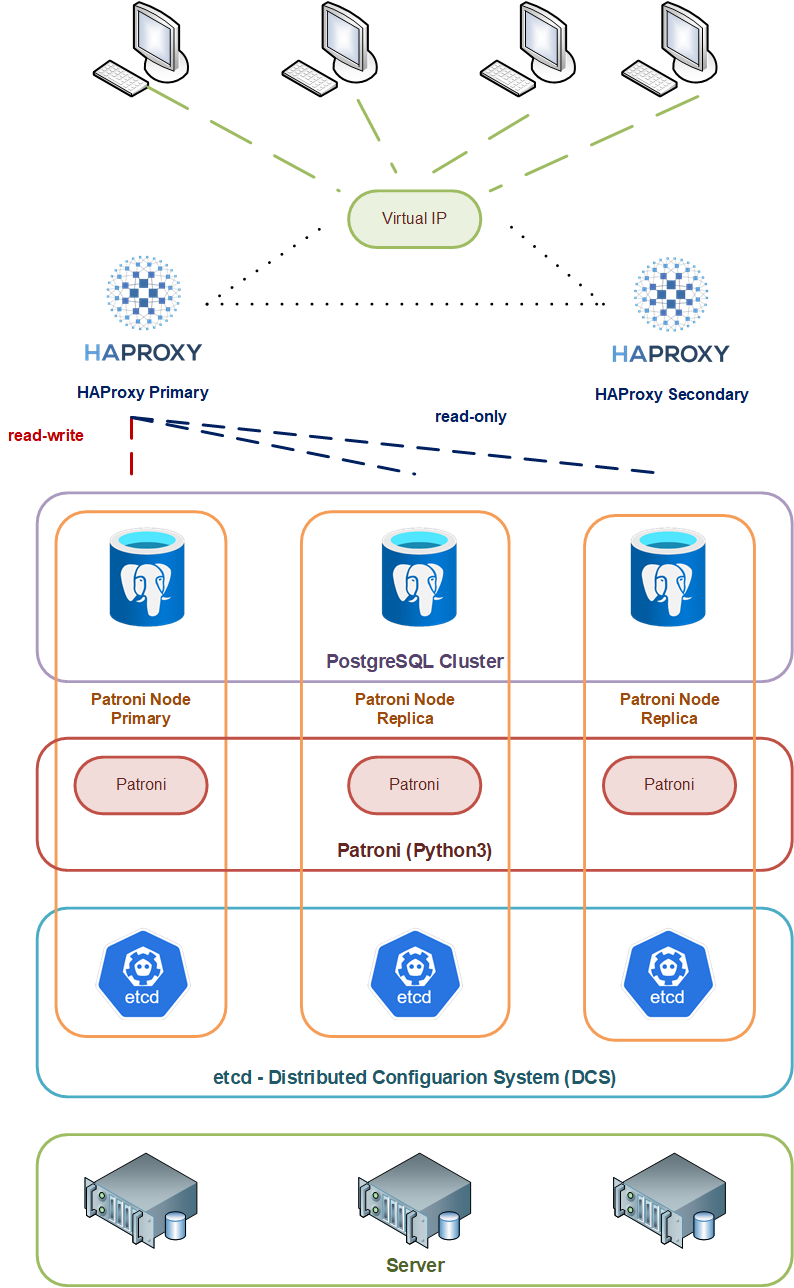
\includegraphics[width=0.7\linewidth]{source/implementation/evaluation/postgresql_ha_solutions/patroni_architecture}
        \caption{Patroni-Architektur}
        \label{fig:patroni-architecture}
    \end{figure}
\end{flushleft}
\begin{flushleft}
    \paragraph{Maintenance}
    Patroni ist ein sehr gepflegtes Projekt, welches die gängigen Community Standards einhält.\\
    Die Details sind im \hyperref[subsec:maintenance_patroni]{Anhang - Maintenance} zu finden.
\end{flushleft}
\begin{flushleft}
    \paragraph{Synergien und Mehrwert}
    Patroni kann nicht nur mit Citus zu einem Distributed / Sharded SQL System umgebaut werden,\\
    es ist auch Kern von StackGres.
\end{flushleft}
\begin{flushleft}
    Damit könnten die API und Skripte in beiden Welten verwendet werden.\\
    Der Aufwand für die Verwaltung und Optimierung würde stark gesenkt.\\
    Projekte wie \texttt{vitabaks / postgresql\_cluster}\cite{HIQVBEPF} bieten zudem die Vorlage für eine noch stärkere Automatisierung.
\end{flushleft}
    \subsubsection{Stackgres mit Citus}
\begin{flushleft} 
Stackgres ist eine PostgreSQL Implementation die dafür vorgesehenen ist, in einem Kubernetes Cluster betrieben zu werden.
\end{flushleft} 
\begin{flushleft}
An sich wäre Stackgres nur eine Implementation von Patroni in Kubernetes inkl. Load Balancer.\\
Nun kommt das Citus-Plugin ins spiel, welches aus einer jeden Monolithischen, Klassischen PostgreSQL Installation eine Distributed SQL Umgebung macht.////
Citus wiederum ist in den Microsoft Konzern eingebettet
\end{flushleft}

\begin{flushleft}
    \paragraph{Architektur}
    \begin{flushleft}
        \subparagraph{Citus Coordinator und Workers}
        \begin{figure}[H]
            \centering
            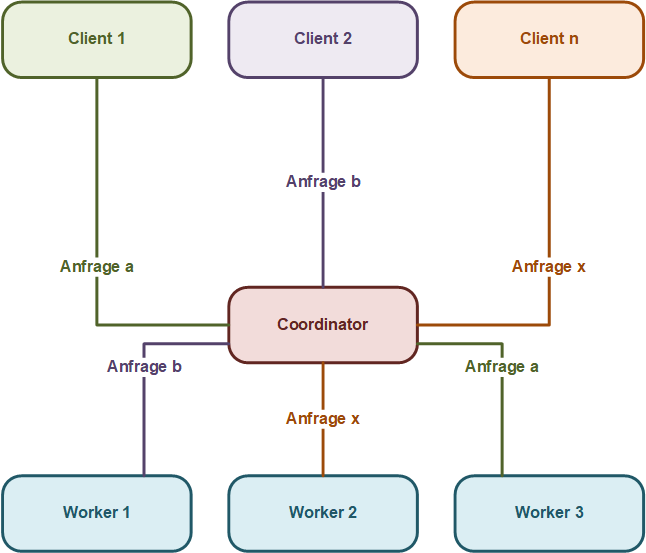
\includegraphics[width=0.75\linewidth]{source/implementation/evaluation/postgresql_ha_solutions/stackgres/citus_coordinator_worker}
            \caption{Citus - Coordinator und Workers}
            \label{fig:citus_coordinator_worker}
        \end{figure}
    \end{flushleft}
    \begin{flushleft}
        \subparagraph{Citus Sharding}
        Citus bietet zwei Sharding-Modelle an.
        \begin{flushleft}
            \textbf{Row-based sharding}
            Beim diesen sharding werden Tabellen anhand einer Distribution Column aufgeteilt. \cite{2Y5FA36C, FDUUL9IM}
        \end{flushleft}
        \begin{flushleft}
            \textbf{Schema-based sharding}
        \end{flushleft}
    \end{flushleft}
\end{flushleft}
\begin{flushleft}
    \paragraph{Maintenance}
    Bei Stackgres gab es im letzten Monat keine wirkliche Bewegung:
    \begin{figure}[H]
        \centering
        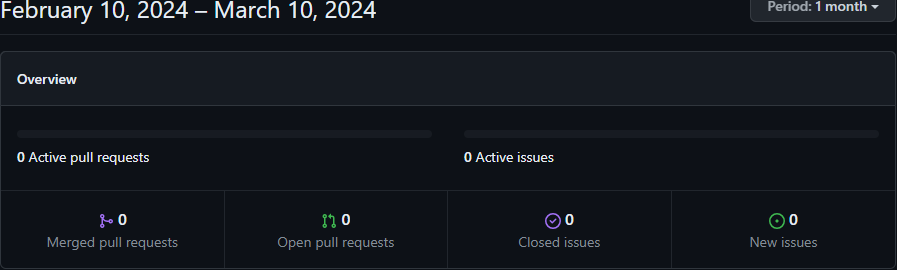
\includegraphics[width=0.75\linewidth]{source/implementation/evaluation/postgresql_ha_solutions/insights/stackgres_citus/pulse_ongres_stackgres}
        \caption{Stackgres - Pulse}
        \label{fig:pulse_ongres_stackgres}
    \end{figure}
    Anders sieht es bei Citus aus, die Firma die mittlerweile zu Microsoft gehört, schliesst Issues rasch und hat eine verhältnissmässig hohe Requstrate:
    \begin{figure}[H]
        \centering
        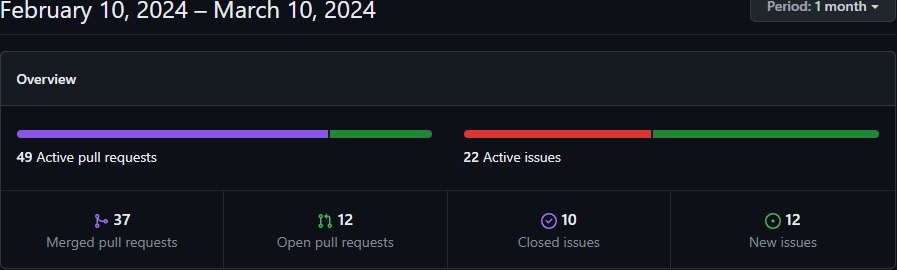
\includegraphics[width=0.75\linewidth]{source/implementation/evaluation/postgresql_ha_solutions/insights/stackgres_citus/pulse_citusdata_citus}
        \caption{Citus - Pulse}
        \label{fig:pulse_citusdata_citus}
    \end{figure}

    Bei Stackgres wird sehr viel Code hinzugefügt oder gelöscht, beim älteren Citus wurden weniger änderungen verzeichnet:
    \begin{figure}[H]
        \centering
        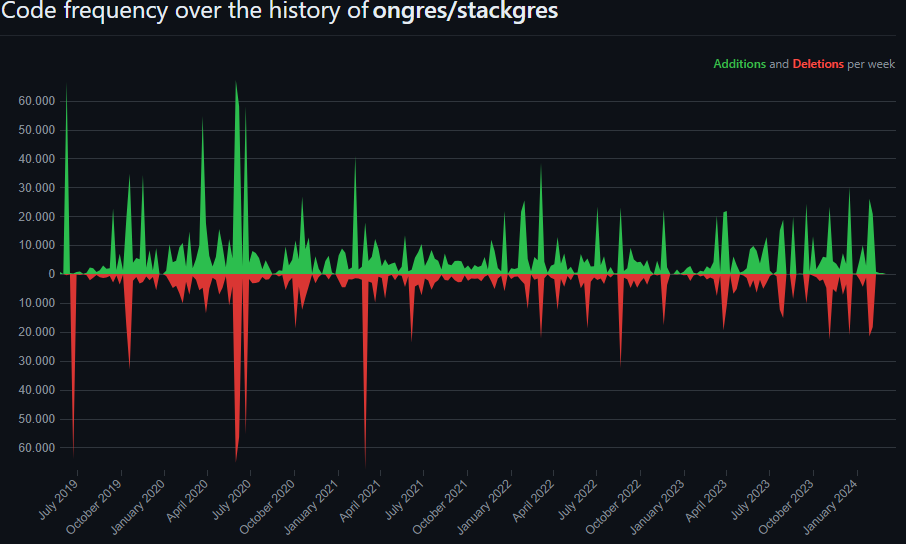
\includegraphics[width=0.75\linewidth]{source/implementation/evaluation/postgresql_ha_solutions/insights/stackgres_citus/code_frequency_ongres_stackgres}
        \caption{Stackgres - Code Frequency}
        \label{fig:code_frequency_ongres_stackgres}
    \end{figure}
    \begin{figure}[H]
        \centering
        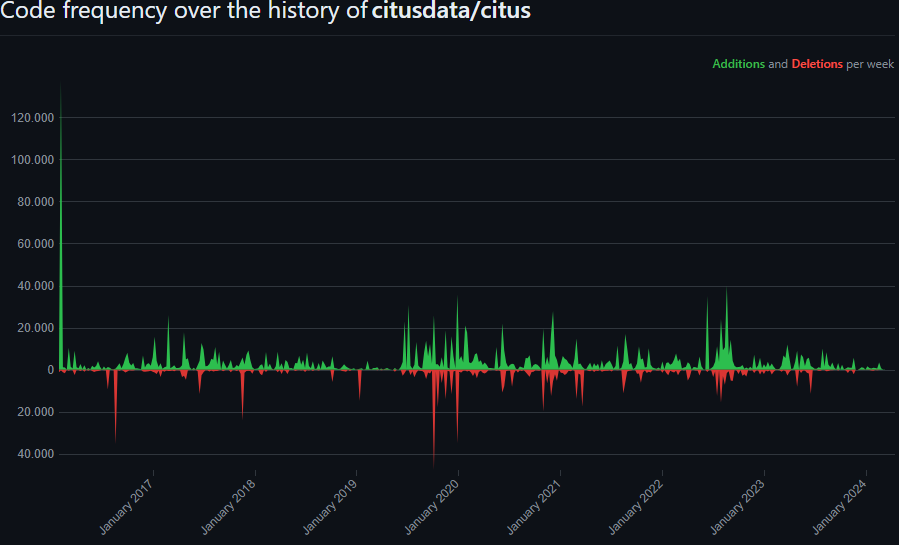
\includegraphics[width=0.75\linewidth]{source/implementation/evaluation/postgresql_ha_solutions/insights/stackgres_citus/code_frequency_citusdata_citus}
        \caption{Citus - Code Frequency}
        \label{fig:code_frequency_citusdata_citus}
    \end{figure}

    Citus legt einen hohen Stellenwert auf die Community-Standars, Stackgres selbst schneidet hier nur Mittelmässig ab:
    \begin{figure}[H]
        \centering
        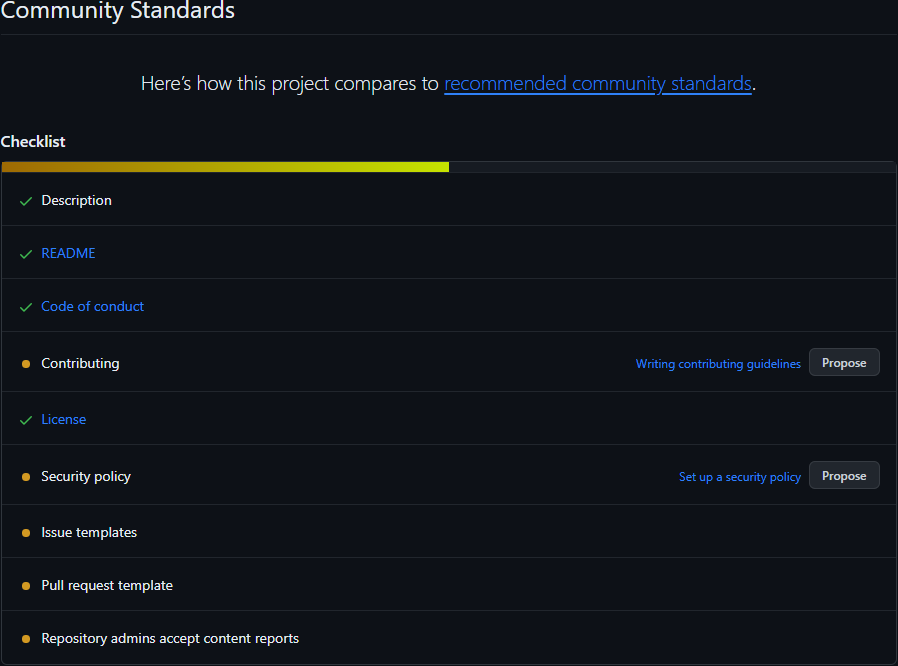
\includegraphics[width=0.75\linewidth]{source/implementation/evaluation/postgresql_ha_solutions/insights/stackgres_citus/stackgres_community_standards}
        \caption{Stackgres - Community Standards}
        \label{fig:stackgres_community_standards}
    \end{figure}
    \begin{figure}[H]
        \centering
        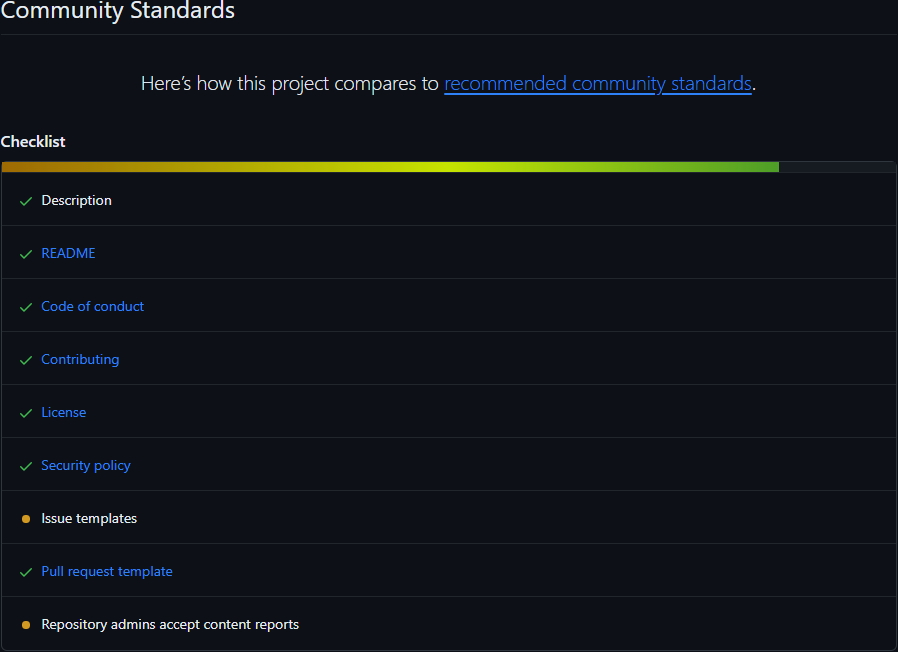
\includegraphics[width=0.75\linewidth]{source/implementation/evaluation/postgresql_ha_solutions/insights/stackgres_citus/citus_community_standards}
        \caption{Citus - Community Standards}
        \label{fig:citus_community_standards}
    \end{figure}

    Die Stackgres Constributors pflegen aktiv Additions ein, löschen Regelmässig und Commiten ebenfalls auf die main-Branch.
    Citus, dessen Repository länger Commited wird, hat weniger bewegung auf die main-Branch.
    \begin{figure}[H]
        \centering
        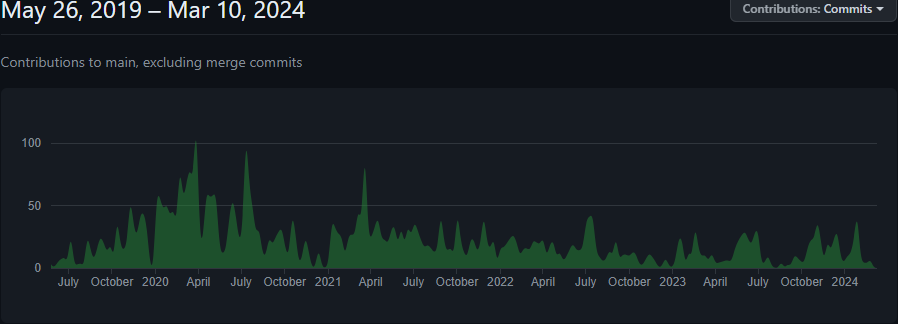
\includegraphics[width=0.75\linewidth]{source/implementation/evaluation/postgresql_ha_solutions/insights/stackgres_citus/contributors_commits_ongres_stackgres}
        \caption{Stackgres - Contributors Commits}
        \label{fig:contributors_commits_ongres_stackgres}
    \end{figure}
    \begin{figure}[H]
        \centering
        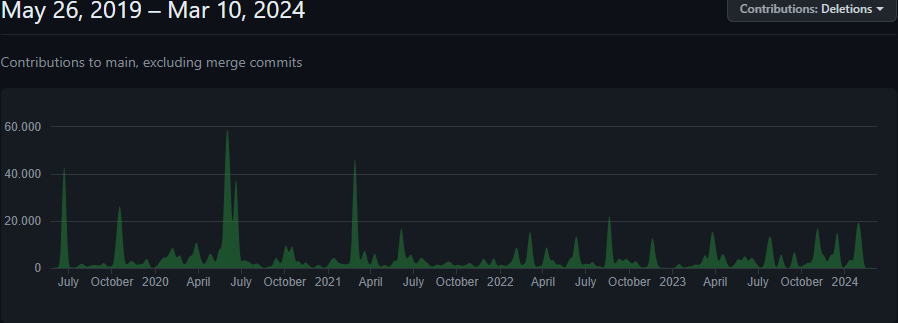
\includegraphics[width=0.75\linewidth]{source/implementation/evaluation/postgresql_ha_solutions/insights/stackgres_citus/contributors_deletations_ongres_stackgres}
        \caption{Stackgres - Contributors Deletations}
        \label{fig:contributors_deletations_ongres_stackgres}
    \end{figure}
    \begin{figure}[H]
        \centering
        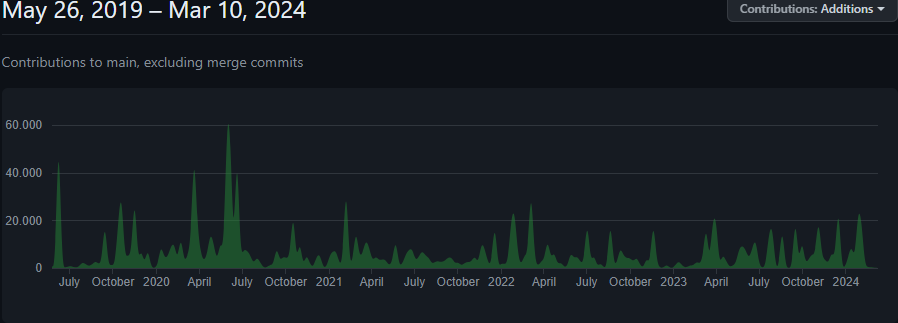
\includegraphics[width=0.75\linewidth]{source/implementation/evaluation/postgresql_ha_solutions/insights/stackgres_citus/contributors_addition_ongres_stackgres}
        \caption{Stackgres - Contributors Additions}
        \label{fig:contributors_addition_ongres_stackgres}
    \end{figure}
    \begin{figure}[H]
        \centering
        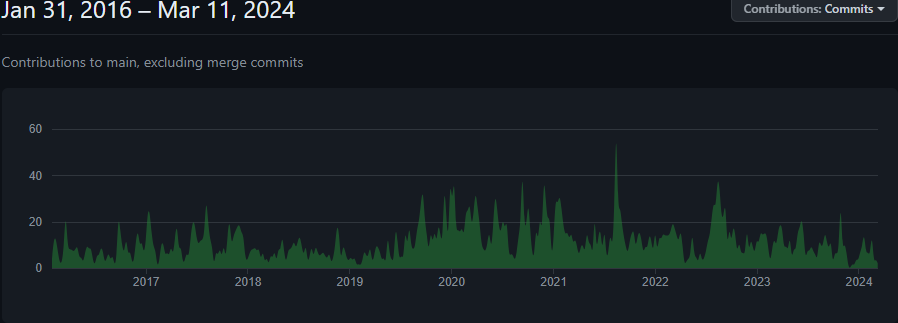
\includegraphics[width=0.75\linewidth]{source/implementation/evaluation/postgresql_ha_solutions/insights/stackgres_citus/contributors_commits_citusdata_citus}
        \caption{Citus - Contributors Commits}
        \label{fig:contributors_commits_citusdata_citus}
    \end{figure}
    \begin{figure}[H]
        \centering
        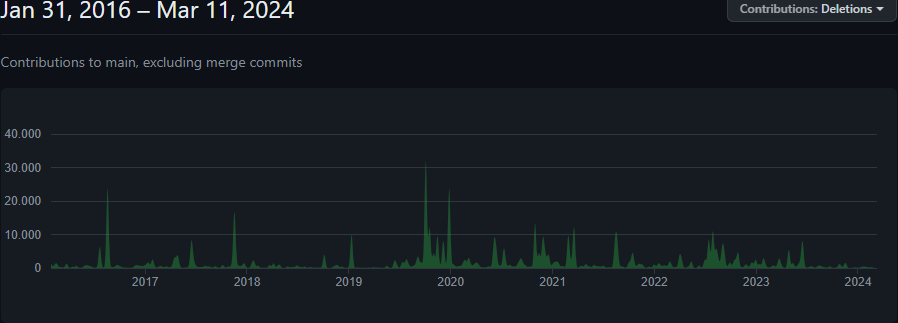
\includegraphics[width=0.75\linewidth]{source/implementation/evaluation/postgresql_ha_solutions/insights/stackgres_citus/contributors_deletations_citusdata_citus}
        \caption{Citus - Contributors Deletations}
        \label{fig:contributors_deletations_citusdata_citus}
    \end{figure}
    \begin{figure}[H]
        \centering
        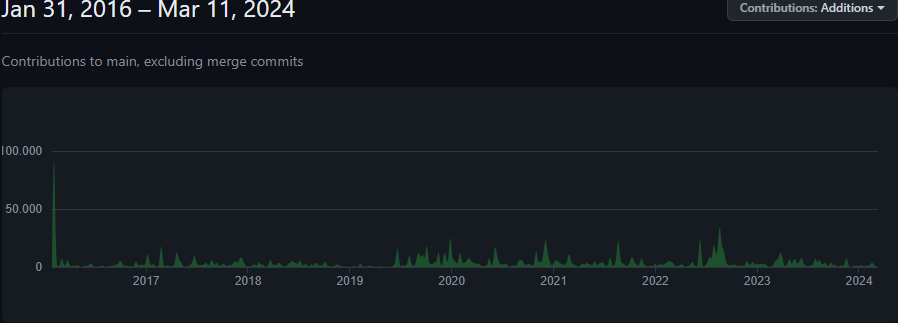
\includegraphics[width=0.75\linewidth]{source/implementation/evaluation/postgresql_ha_solutions/insights/stackgres_citus/contributors_additions_citusdata_citus}
        \caption{Citus - Contributors Additions}
        \label{fig:contributors_additions_citusdata_citus}
    \end{figure}

    Gerade Ende Januar gab es bei Stackgres eine grössere Anzahl Commits, anhand der statistik wird ersichtlich, dass i.d.R. einmal pro Monat grössere Mengen an Commits eingespielt werden.
    Bei Citus gibt es ebenfalls Regelmässig grössere Mengen an Commits, allerdings scheint bei citusdata mehr mit kürzeren Sprints gearbeitet zu werden als bei ongres denn die Commits sind Regelmässiger:
    \begin{figure}[H]
        \centering
        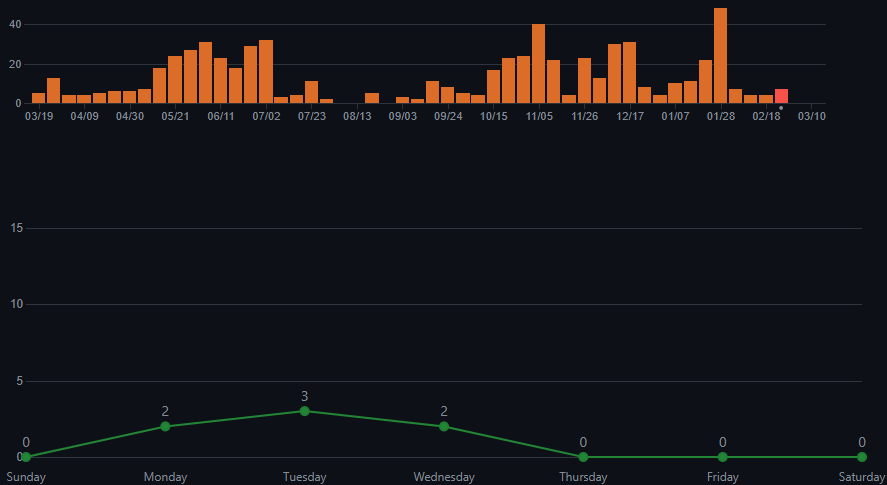
\includegraphics[width=0.75\linewidth]{source/implementation/evaluation/postgresql_ha_solutions/insights/stackgres_citus/commit_activity_ongres_stackgres}
        \caption{Stackgres - Commit Activity}
        \label{fig:commit_activity_ongres_stackgres}
    \end{figure}
    \begin{figure}[H]
        \centering
        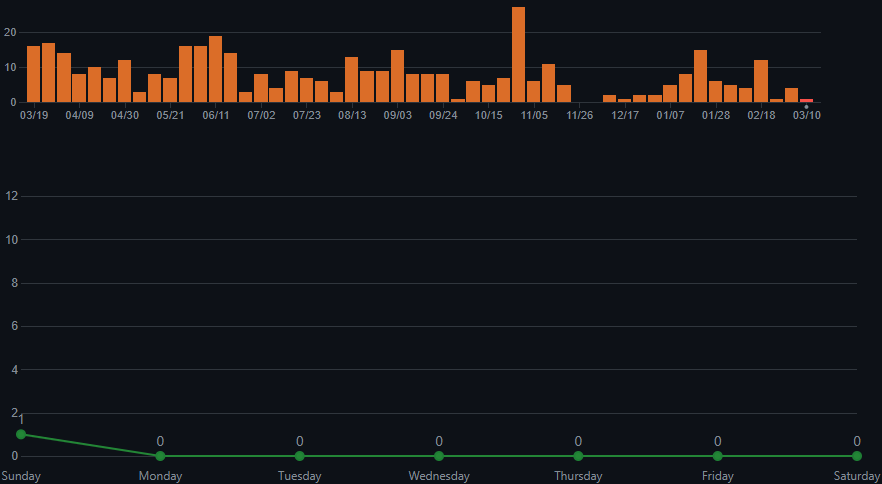
\includegraphics[width=0.75\linewidth]{source/implementation/evaluation/postgresql_ha_solutions/insights/stackgres_citus/commit_activity_citusdata_citus}
        \caption{Citus - Commit Activity}
        \label{fig:commit_activity_citusdata_citus}
    \end{figure}

    In letzter Zeit haben nur ongres, der Entwickler von Stackgres, als auch citusdata, grössere Commits auf das Repository gefahren.
    Andere grössere Entwickler wie EnterpriseDB sind abwesend.
    \begin{figure}[H]
        \centering
        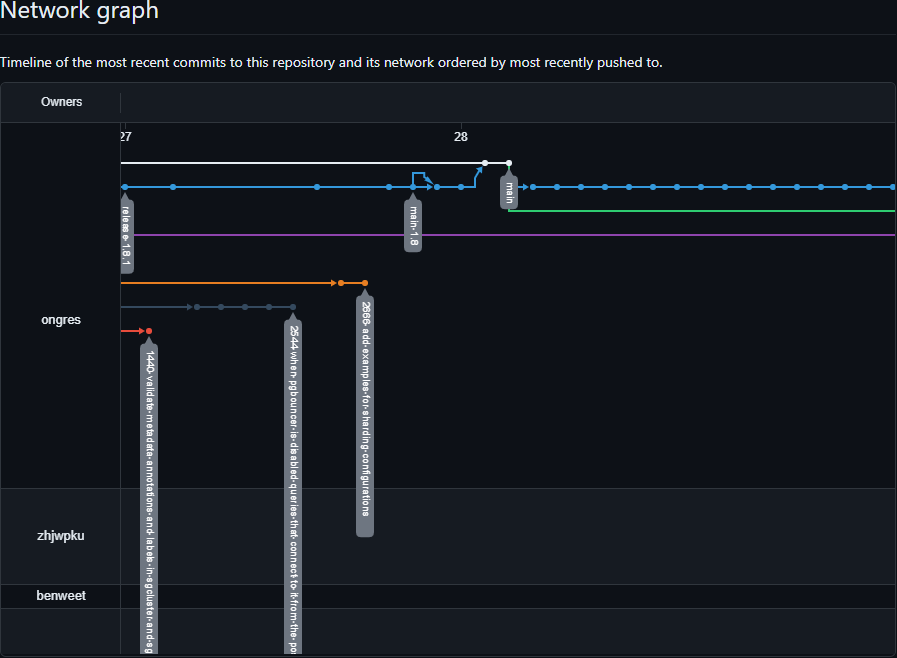
\includegraphics[width=0.75\linewidth]{source/implementation/evaluation/postgresql_ha_solutions/insights/stackgres_citus/network_graph_ongres_stackgres}
        \caption{Stackgres - Network Graph}
        \label{fig:network_graph_ongres_stackgres}
    \end{figure}
    \begin{figure}[H]
        \centering
        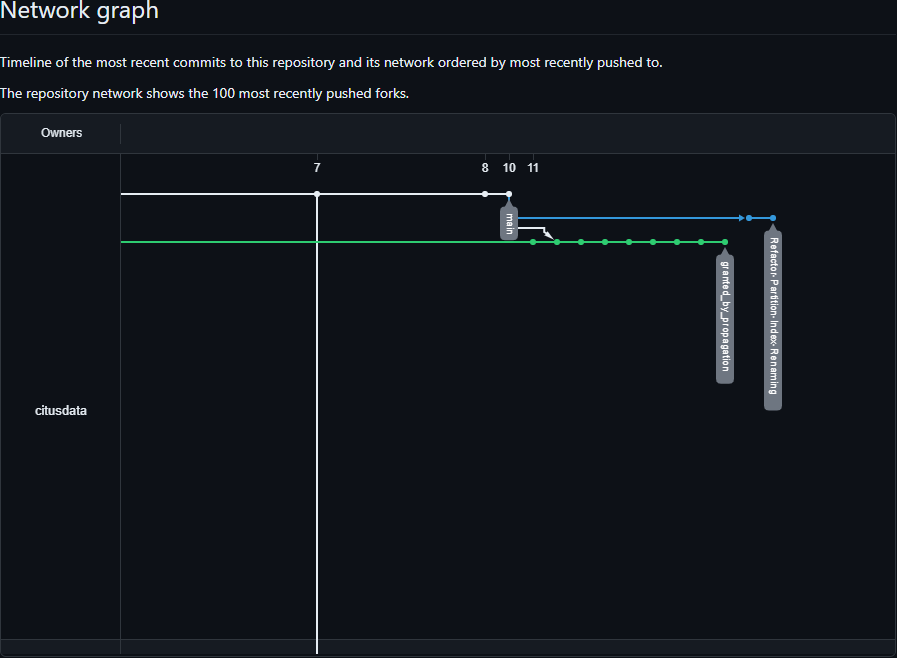
\includegraphics[width=0.75\linewidth]{source/implementation/evaluation/postgresql_ha_solutions/insights/stackgres_citus/network_graph_citusdata_citus}
        \caption{Citus - Network Graph}
        \label{fig:network_graph_citusdata_citus}
    \end{figure}

\end{flushleft}
    %! Author = gramic
%! Date = 22.04.24

% Preamble
\begin{flushleft}
    \subsection{YugabyteDB}
    \label{subsec:appendix_testing_yugabytedb}
    Zum einen kann der Fehler irgendwann auftreten.\\
    In diesem Fall wird erst im Log die Fehlermeldung geworfen, dass die Zeitdifferenz zu gross ist:
    \begin{figure}[H]
        \centering
        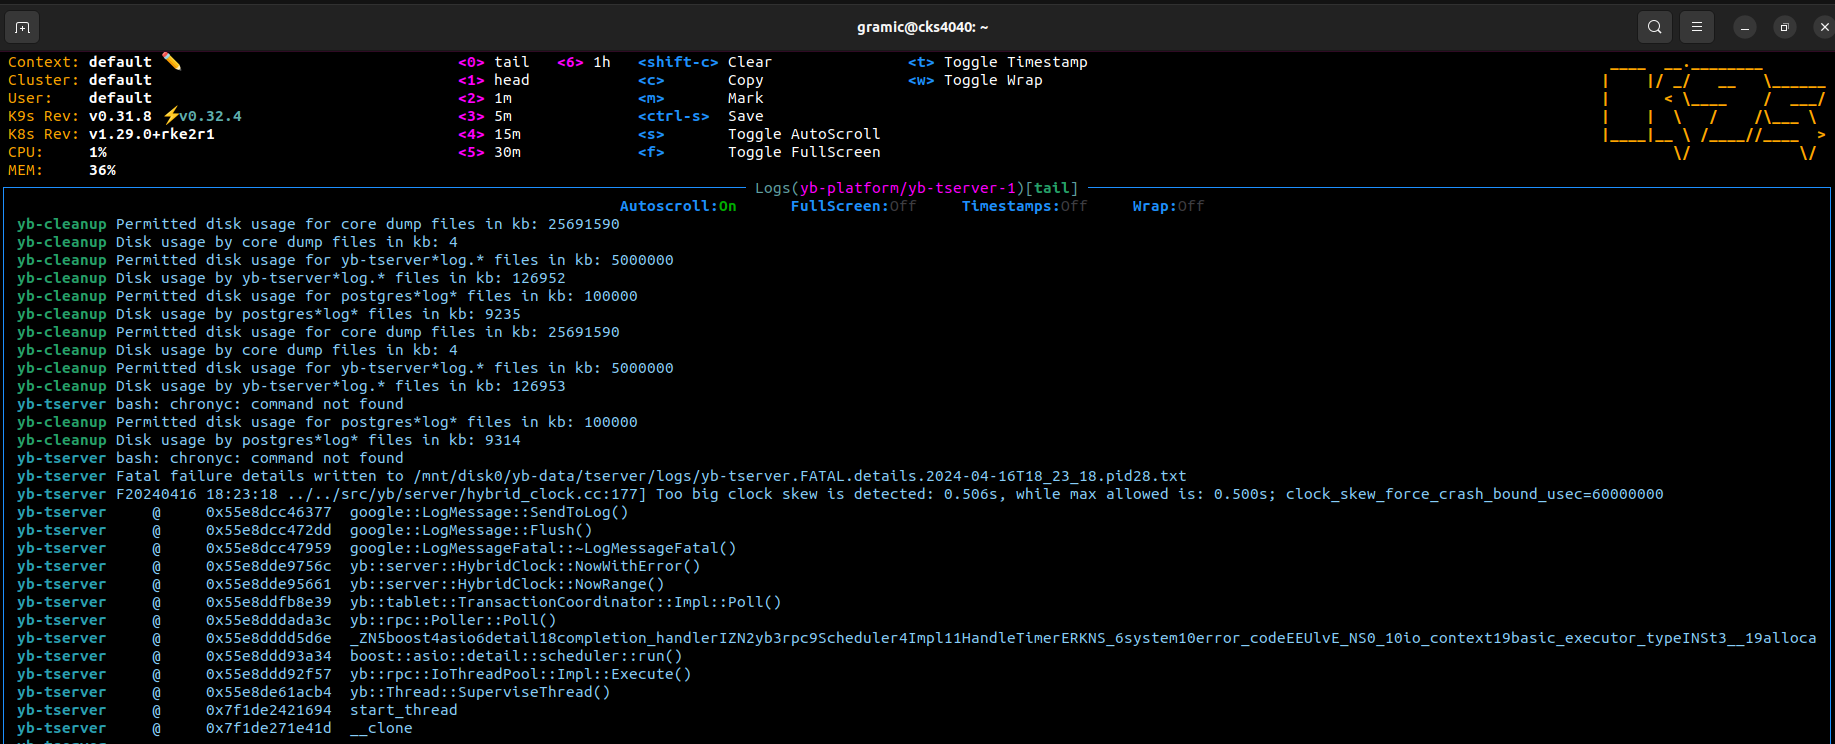
\includegraphics[width=1\linewidth]{source/appendix/evaluation_testing/yugabytedb_too_big_clock_skew_is_detected}
        \caption{YugabyteDB - Too big clock skew is detected}
        \label{fig:yugabytedb_too_big_clock_skew_is_detected}
    \end{figure}
    Eine Folge ist, dass kein neuer Leader bestimmt werden kann:
    \begin{figure}[H]
        \centering
        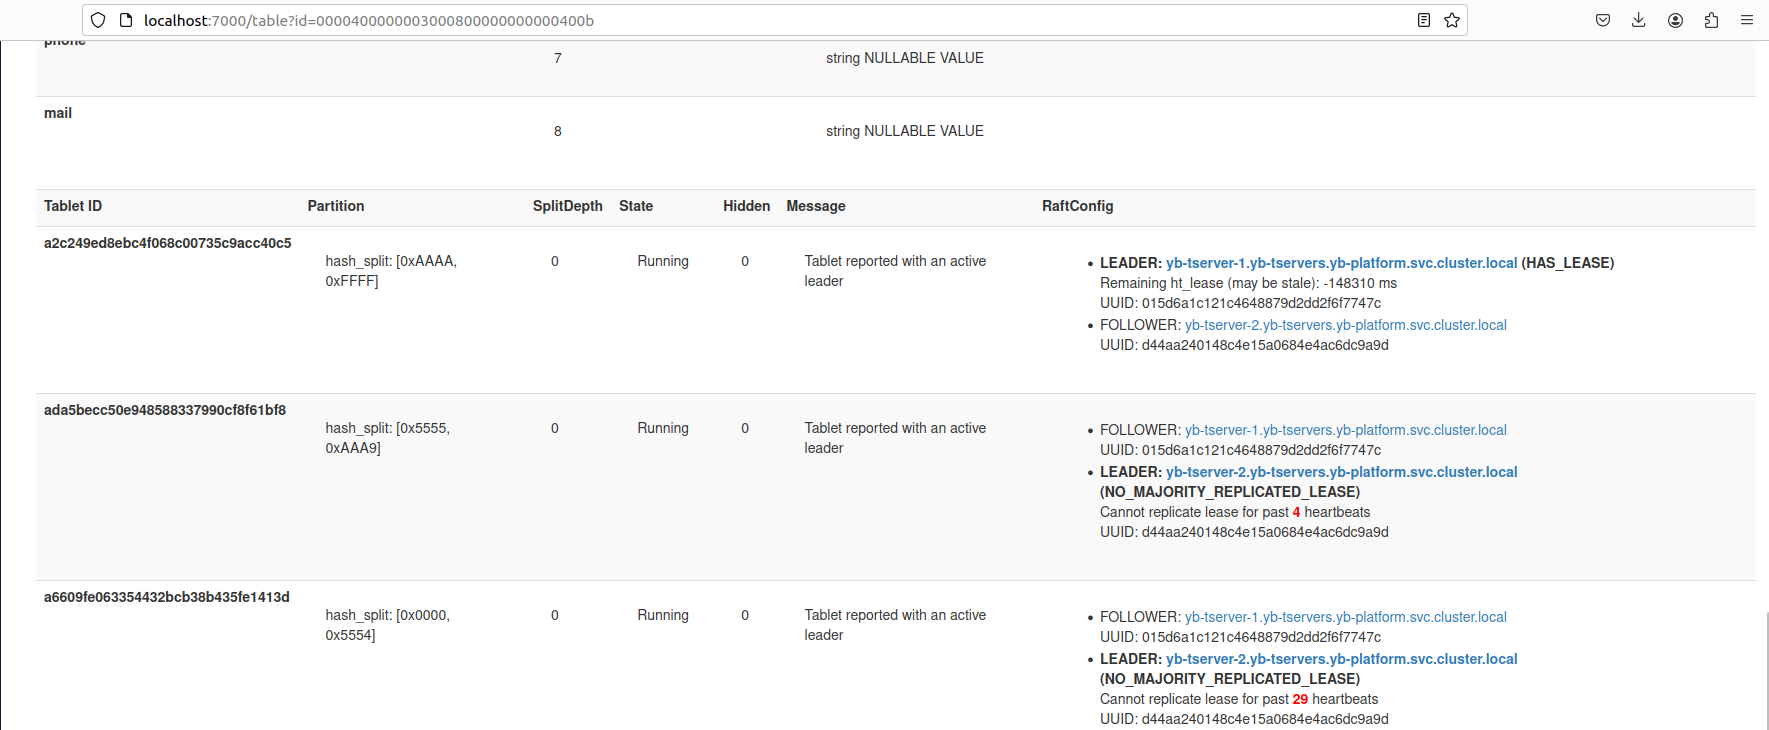
\includegraphics[width=1\linewidth]{source/appendix/evaluation_testing/yugabytedb_tablet_leader_lease}
        \caption{YugabyteDB - Tablet Leader - No Lease}
        \label{fig:yugabytedb_tablet_leader_lease}
    \end{figure}
    Als nächstes wird der komplette \texttt{tserver} in einem \texttt{CrashLoopBackOff} fallen:
    \begin{figure}[H]
        \centering
        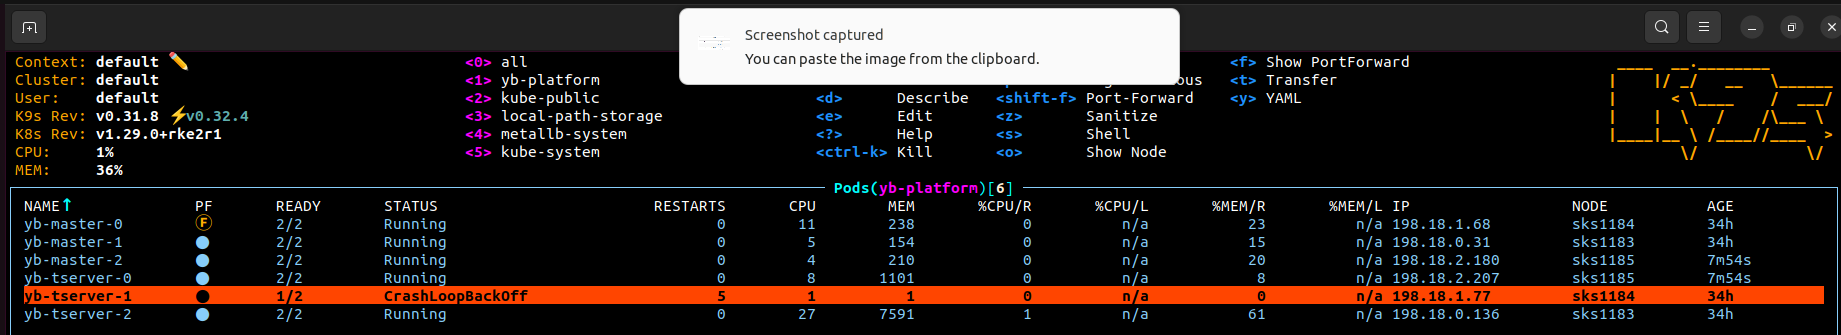
\includegraphics[width=1\linewidth]{source/appendix/evaluation_testing/yugabytedb_crashloopbackoff}
        \caption{YugabyteDB - CrashLoopBackOff}
        \label{fig:yugabytedb_crashloopbackoff}
    \end{figure}
    Der ganze Cluster an sich aber bleibt arbeitsfähig.
\end{flushleft}
\begin{flushleft}
    Anders sieht es aus, wenn auch \texttt{tmaster}-Nodes von Start weg betroffen sind.\\
    Es werden aber primär nur die Logs überall geschrieben:
    \begin{figure}[H]
        \centering
        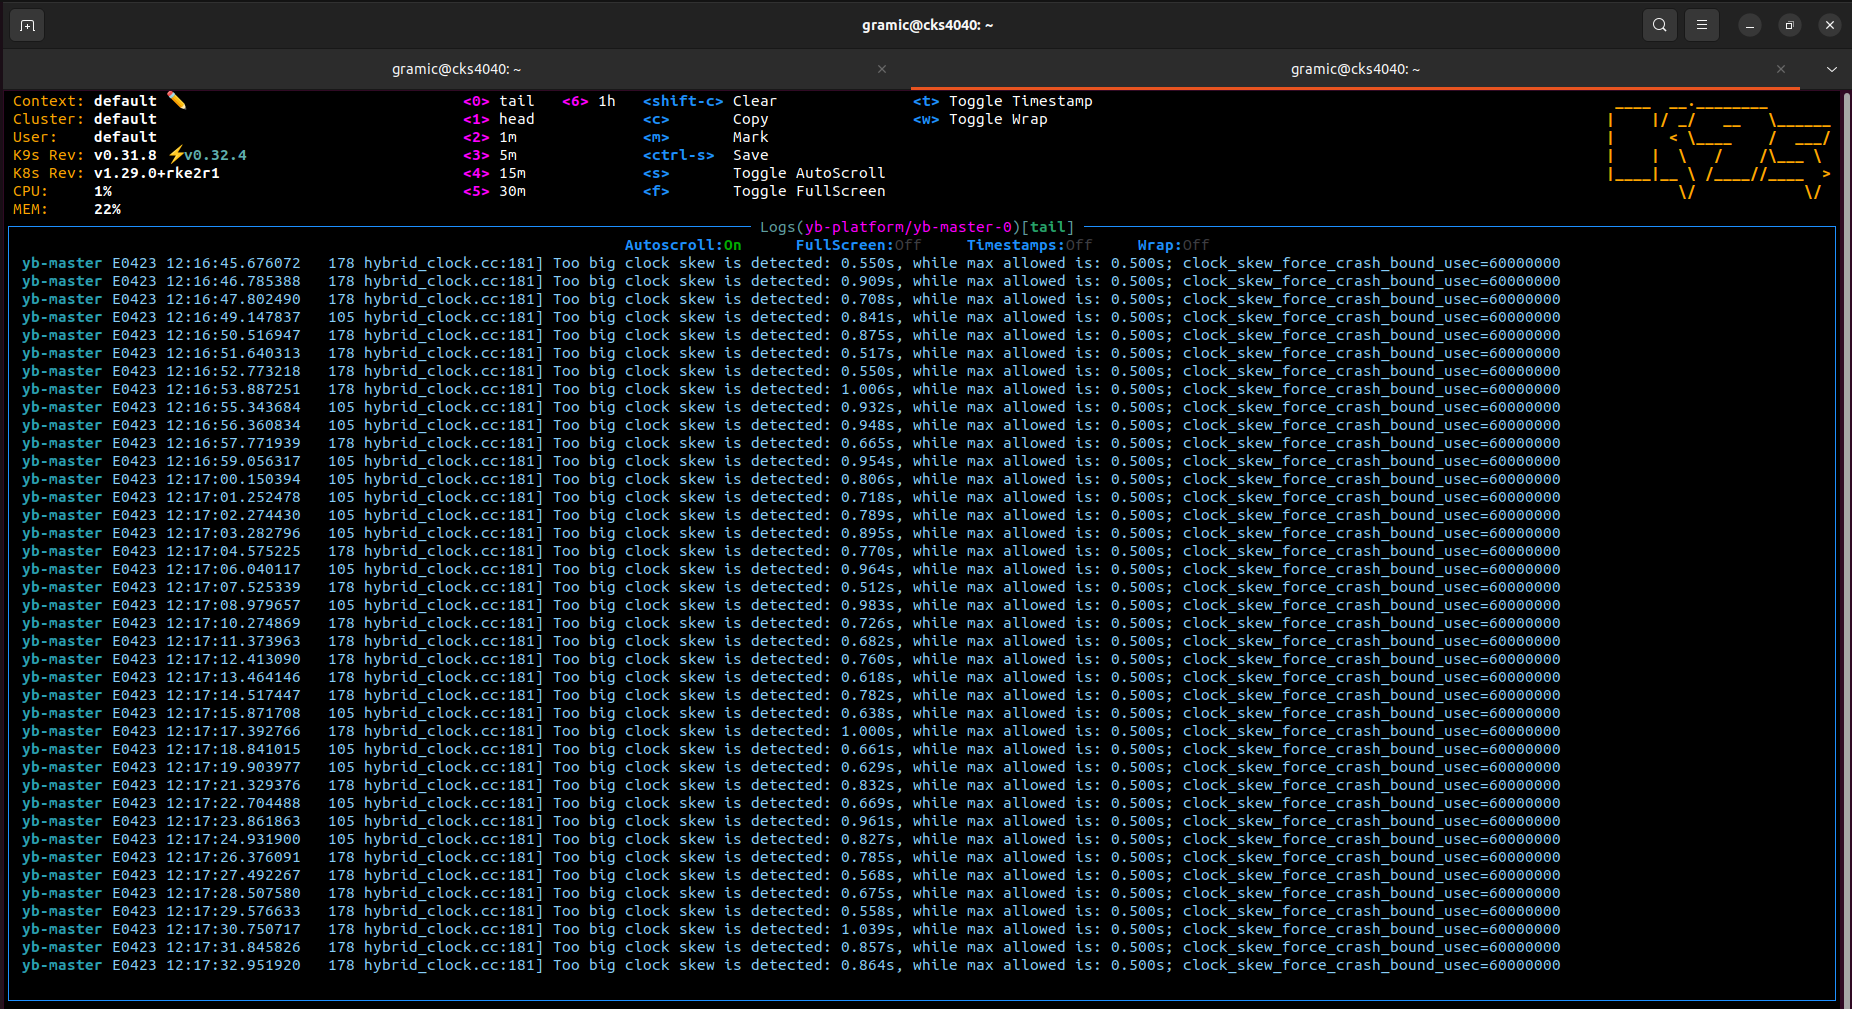
\includegraphics[width=1\linewidth]{source/appendix/evaluation_testing/yugabytedb_yb-tmaster-0_sks1184_clock_error}
        \caption{YugabyteDB - Too big clock skew is detected - tmaster}
        \label{fig:yugabytedb_yb-tmaster-0_sks1184_clock_error}
    \end{figure}
    \begin{figure}[H]
        \centering
        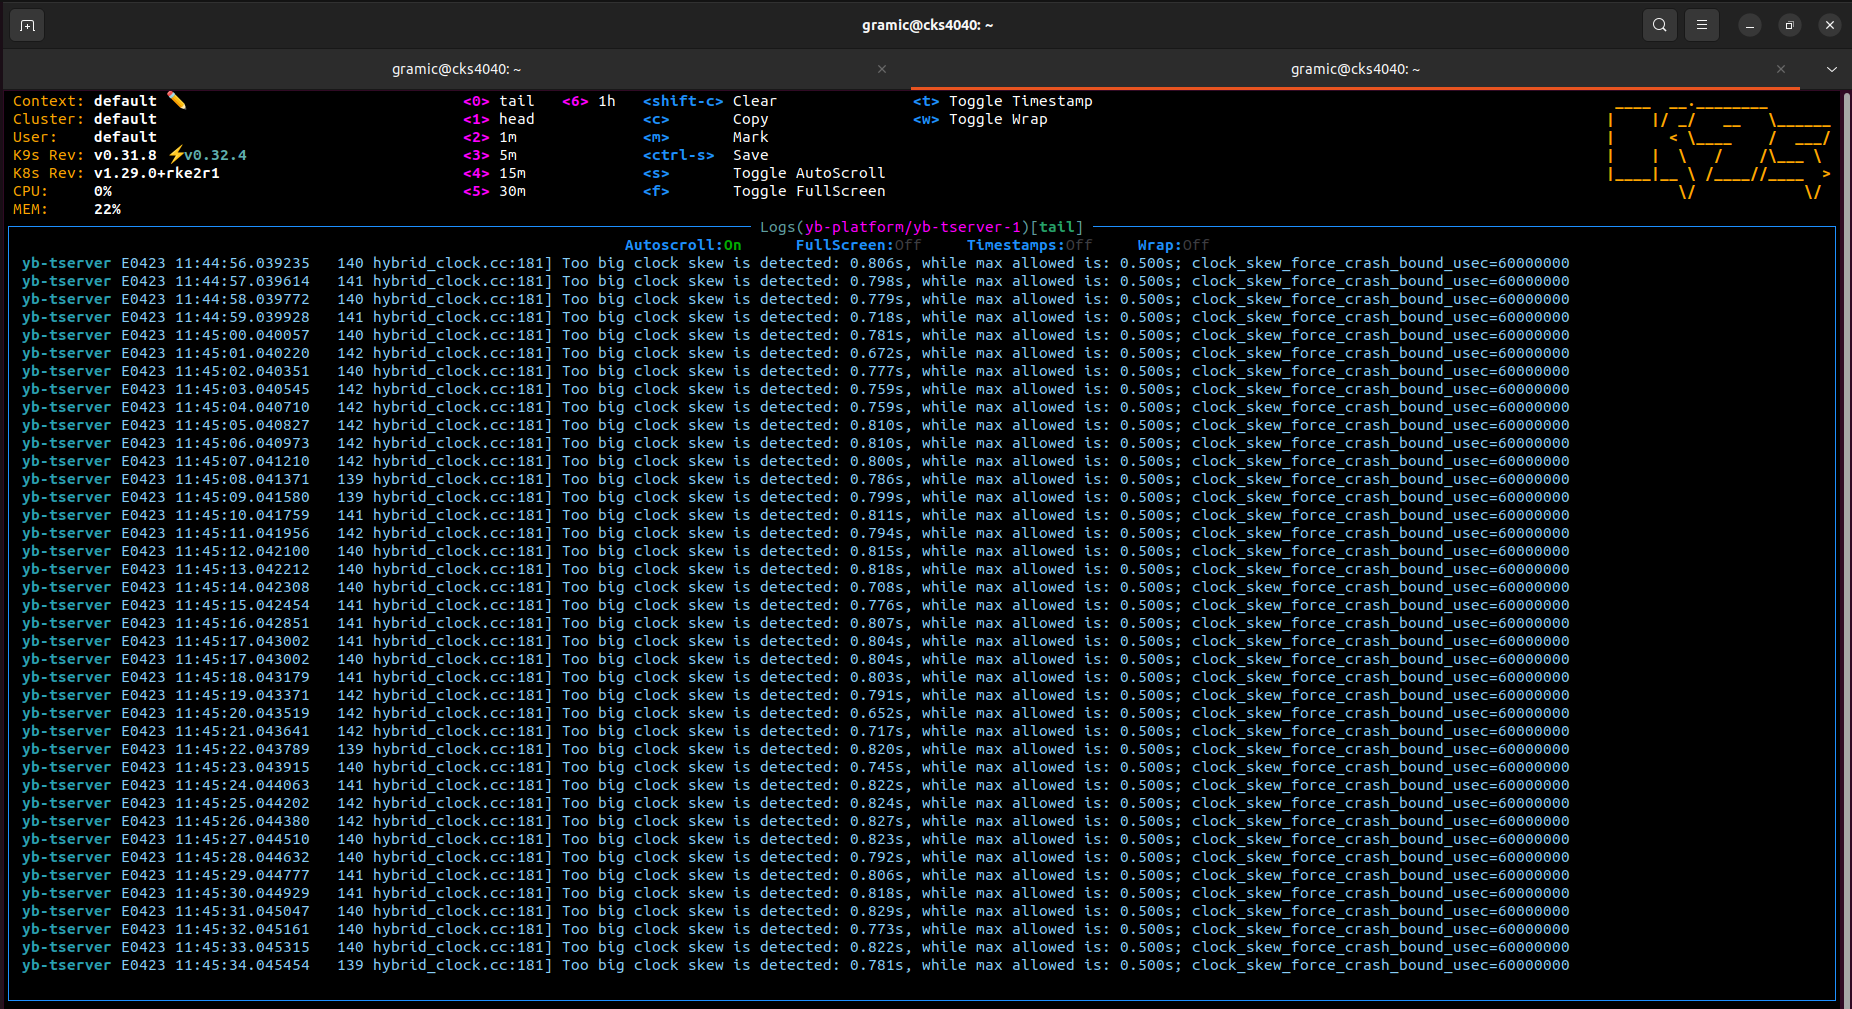
\includegraphics[width=1\linewidth]{source/appendix/evaluation_testing/yugabytedb_yb-tserver-1_sks1184_clock_error}
        \caption{YugabyteDB - Too big clock skew is detected - tserver}
        \label{fig:yugabytedb_yb-tserver-1_sks1184_clock_error}
    \end{figure}
%    \begin{figure}[H]
%        \centering
%        \subfloat[yb-tmaster-0]{{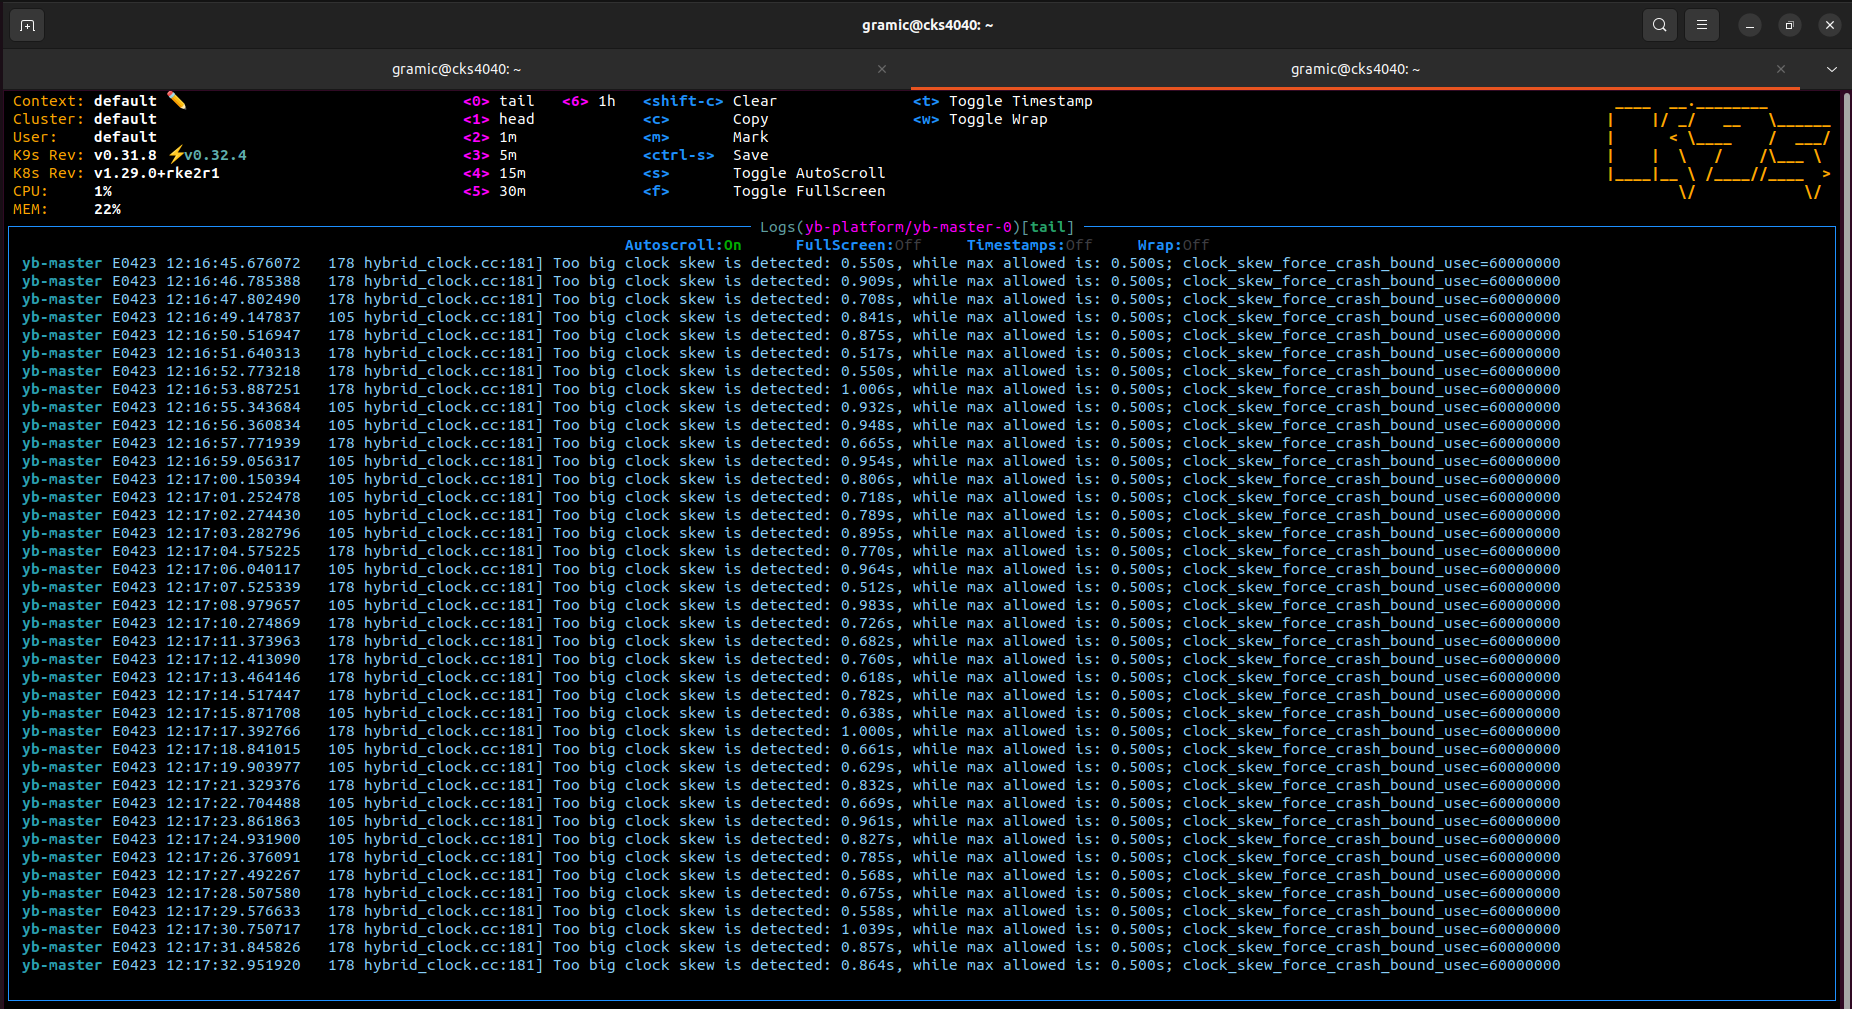
\includegraphics[width=0.47\linewidth]{source/appendix/evaluation_testing/yugabytedb_yb-tmaster-0_sks1184_clock_error} }}%
%        \qquad
%        \subfloat[yb-tserver-1]{{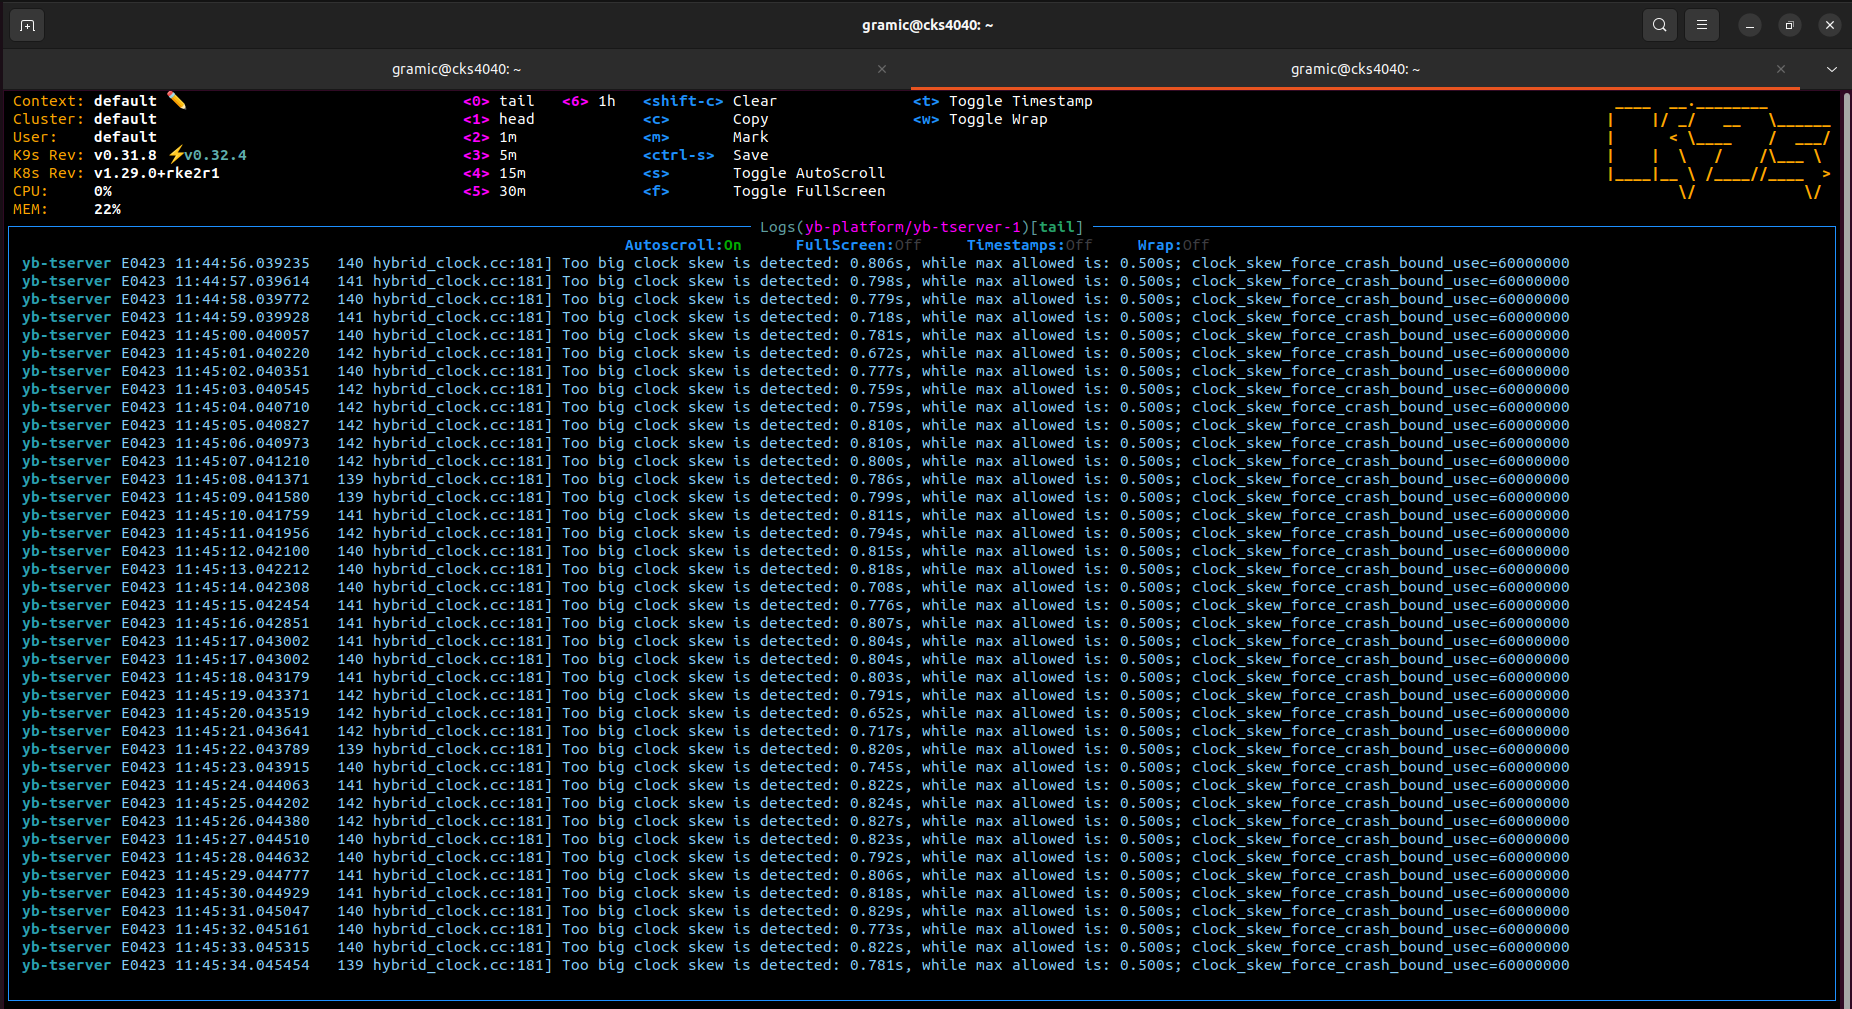
\includegraphics[width=0.47\linewidth]{source/appendix/evaluation_testing/yugabytedb_yb-tserver-1_sks1184_clock_error} }}%
%        \caption{YugabyteDB - Too big clock skew is detected - Node}
%        \label{fig:yugabytedb_sks1184_clock_error}
%    \end{figure}
    YugabyteDB erlaubt in so einem Fall keine Zugriffe mehr auf den Cluster.\\
    So wird verhindert, dass der Cluster korrumpiert wird.
\end{flushleft}
    %! Author = gramic
%! Date = 11.03.24

% Preamble
\begin{flushleft}
    \subsection{Vorauswahl}
    Folgende Lösungen werden nicht evaluiert, sondern bereits zu Beginn ausgeschieden:
    \begin{table}[H]

\resizebox{\columnwidth}{!}{%

\begin{tabular}{rlll}
\toprule
Nr. & Lösung & Status & Begründung \\
\midrule
1 & KSGR-Lösung & Vorausgeschieden & \begin{tabular}[c]{@{}l@{}}Hat nur einen Standy / Replika-Node.\\Failover Funktioniert nur bei kleineren Datenmengen wirklich in einer vernüftigen Zeit.\end{tabular} \\
2 & pgpool-II & Vorausgeschieden & \begin{tabular}[c]{@{}l@{}}pgpool-II hat kein GitHub-Repository und bietet daher keine vergleichswerte mittels Github Insights.\end{tabular} \\
3 & pg\_auto\_failover & Vorausgeschieden & \begin{tabular}[c]{@{}l@{}}pg\_auto\_failover würde zwar Citus-Support bieten,\\allerdings gibt es keine gut dokumentierte Implementation für Kubernetes.\\Erfüllt daher das Kriterium für die Synergien nicht\end{tabular} \\
4 & CloudNativePG & Vorausgeschieden & \begin{tabular}[c]{@{}l@{}}CloudNativePG ist keine vollständige Cloud Native Lösung.\\Mittels Citus könnte sogar eine Distributed SQL Lösung implementiert werden.\\Die Grundarchitektur bleibt aber Monolithisch mit einem Primary und Replikas.\\Und da kein Benefit in Form von Synergien vorhanden sind,\\fällt CloudNativePG raus.\end{tabular} \\
8 & Citus row-based-sharding & Vorausgeschieden & \begin{tabular}[c]{@{}l@{}}Citus row-based-sharding wäre Hocheffizient\\wenn es um Ressourcenverteilung geht und zudem echtes Sharding.\\Allerdings setzt es anpassungen an den Tabellen der Applikationen voraus.\\Das KSGR ist allerdings kein Softwarehaus\\und kann keine Forks durchführen,\\auch weil viele Applikationen zertifiziert sein müssen.\\Scheitert daher an der Machbarkeit\end{tabular} \\
\bottomrule
\end{tabular}
}
\caption{Vorauswahl - Ausgeschieden} \label{predecision_out}
\end{table}


    Entsprechend werden nur noch nachfolgende Lösungen genauer betrachtet:
    \begin{table}[H]

\resizebox{\columnwidth}{!}{%

\begin{tabular}{rlll}
\toprule
Nr. & Lösung & Status & Begründung \\
\midrule
4 & Patroni & Evaluation & \begin{tabular}[c]{@{}l@{}}Patroni kann als Monolithisches System genutzt werden,\\ist aber auch Kern von Stackgres.\\Die API und Skripte können also in beiden Welten verwendet werden\end{tabular} \\
5 & Stackgres mit Citus & Evaluation & \begin{tabular}[c]{@{}l@{}}Bietet eine einfache und kompakte Möglichkeit für ein Distributed SQL System.\\Da Patroni unter der Haube ist,\\kann die API und sonstige Skripte auch auf einem Monolithischen System eingesetzt werden.\end{tabular} \\
6 & Yugabyte-DB & Evaluation & \begin{tabular}[c]{@{}l@{}}Ist eine reine Distributed SQL Lösung und ist Vollständig Cloud Native.\end{tabular} \\
\bottomrule
\end{tabular}
}
\caption{Vorauswahl - Evaluation} \label{predecision_in}
\end{table}

\end{flushleft}
\end{flushleft}